\documentclass[UTF8, fontset=macnew, a4paper, 12pt]{ctexart}

\usepackage{geometry}
\geometry{top=2.5cm, bottom=2.5cm, left=2.5cm, right=2.5cm}
\usepackage{amsmath, amssymb}
\usepackage{booktabs}
\usepackage{multirow}
\usepackage{graphicx}
\usepackage{caption}
\usepackage{xcolor}
\usepackage{float}
\usepackage{enumitem}
\usepackage{fancyhdr}
\usepackage{setspace}
\usepackage{pifont}
\usepackage[hidelinks]{hyperref}

\graphicspath{{../output/figures/}}
\captionsetup{font=small, labelfont=bf, labelsep=quad}
\setlist{itemsep=2pt, parsep=0pt, topsep=4pt}
\onehalfspacing

\ctexset{
  section/format = \raggedright\zihao{4}\bfseries,
  section/name   = {},
  section/number = \chinese{section}、,
  subsection/format = \raggedright\zihao{5}\bfseries,
  subsection/number = \chinese{subsection},
  subsection/aftername = 、,
  subsubsection/format = \raggedright\normalsize\bfseries,
}
\renewcommand{\thesection}{\chinese{section}}
% 交叉引用子節時補上節次，否則 \ref 只印出「三」而無從判斷屬於哪一節。
% \p@subsection 是 LaTeX 寫入 .aux 時加在 \thesubsection 前的前綴。
\renewcommand{\thesubsection}{\chinese{subsection}}
\makeatletter
\renewcommand{\p@subsection}{\thesection 之}
\makeatother
\setcounter{secnumdepth}{2}   % subsubsection 不編號（標題已自帶（一）（二））

\pagestyle{fancy}
\fancyhf{}
\fancyhead[L]{\small 小人口 Lee-Carter 模型的參數分層診斷與估計}
\fancyhead[R]{\small 碩士論文進度報告（1006）}
\fancyfoot[C]{\small \thepage}
\renewcommand{\headrulewidth}{0.4pt}

% U+2460~2463（\cn{1}~\cn{4}）不在 xeCJK 認定的 CJK 範圍內，會落到拉丁字型而缺字，
% 故改用 pifont 的圈號。
\newcommand{\cn}[1]{\ding{\number\numexpr171+#1\relax}}
\newcommand{\edag}{e_0^{\dagger}}
\newcommand{\LCe}{\mathrm{LC}e^{\dagger}}

\begin{document}

\begin{center}
{\zihao{3}\bfseries 小人口 Lee-Carter 模型的參數分層診斷與估計}\\[4pt]
{\zihao{5} —— 從資料的分布，決定哪些參數可估、該用哪個估計量}\\[4pt]
{\zihao{5}\textbf{第四版（1006）}：依 EDA 佈局與穩健方法架構重組，收斂研究主軸}\\[12pt]
{\zihao{5} （林子立）\quad 指導教授：余清祥\,教授}\\[4pt]
{\zihao{5} 國立政治大學統計學系}\\[4pt]
{\zihao{5} 中華民國 115 年 9 月 26 日}
\end{center}

\vspace{6pt}
\begin{center}
\begin{minipage}{0.92\textwidth}
\small
\textbf{摘要}\par\vspace{4pt}
我國多數鄉鎮市區的單一性別人數不足五萬，Lee-Carter 模型的參數在此規模下
出現有方向的偏誤。本文指出三個參數因\textbf{不同機制}失效：$\alpha_x$ 源於
零格替代與對數轉換、漂移項源於等權重分解對異質變異的敏感、$\beta_x$ 則受
訊噪比限制而在相變門檻以下不可還原。三者皆可由四項\textbf{不需真值的事前
診斷}辨認，並分別以偏誤減少、資訊加權與經驗貝氏收縮對應處理。\par\vspace{6pt}
\textbf{關鍵詞}：小區域估計、Lee-Carter 模型、偏誤診斷、偏誤減少、
經驗貝氏收縮、預測區間
\end{minipage}
\end{center}

\vspace{10pt}

\section{緒論}

\subsection{研究背景：鄉鎮市區生命表的空白}

平均餘命是衡量地區發展的核心指標，其估計須以各年齡的死亡率為基礎。然而
我國官方僅公布全國與縣市層級的簡易生命表，鄉鎮市區層級付之闕如。原因不在
資料不全，而在\textbf{樣本規模}：368 個鄉鎮市區中有 217 個（59\%）的單一
性別人數在兩萬以下、299 個（81\%）少於五萬人，此等規模下年齡別死亡率的
觀測值震盪劇烈，甚至經常出現死亡人數為零的年齡組（余清祥等 2025）。

問題不止於估計值不穩。Wang et al.（2018）與余清祥等（2021）發現，LC 模型
的年齡參數在人數減少時會出現\textbf{有方向的偏誤}，且此偏誤在人數二十萬
以下時特別明顯。偏誤與變異數的差別至關重要：變異數大可藉由增加資料或重複
抽樣察覺，偏誤卻會在所有樣本上朝同一方向偏移，單看估計結果無從發現。

\subsection{Lee-Carter 模型的成功，以及它隱含的假設}

Lee and Carter（1992）以一組簡潔的雙線性結構描述死亡率的時間變化，三十年
來成為死亡率推估的標準工具。Basellini et al.（2023）在其三十週年回顧中
列出該模型成功的四項理由：\textbf{結構簡潔}，單一時間指標即可導出全年齡的
預測；\textbf{時間指標在多數應用中近乎線性}，故可用隨機漫步含漂移項外推；
\textbf{隨機架構可導出機率預測區間}；以及\textbf{純粹外推、不需主觀判斷}，
因而具有可重複性。這四項優點在國家級人口上已被反覆驗證。

\textbf{因此，本文要檢驗的不是 LC 模型是否正確，而是它在何種條件下適用。}

回答這個問題的關鍵，在於指出一個平常不被明說的前提。LC 模型的標準解法是
對中心化的對數死亡率矩陣取奇異值分解，而\textbf{奇異值分解等價於無加權的
最小平方}，因此隱含了\textbf{同質變異與常態誤差}的高斯架構——每一個
年齡--年份的格子，在目標函數裡被賦予相同的權重。

這個前提在國家級人口上大致成立。本文表~\ref{tab:datadesc} 顯示，全國女性
2001--2024 年的 528 個格子中，單格死亡數最少亦有 37 人、中位數 1{,}201 人，
零死亡格為 0。但在單一性別不足兩萬的鄉鎮市區，同樣的 528 個格子中平均有
206 格為零。\textbf{同質變異假設在此不是略有偏差，而是完全失效。}

\subsection{從資料的分布，看假設如何失效}\label{sec:intro-eda}

前述主張若只靠引文支持，僅能證明別人也這麼說。本文因此先以\textbf{四項
不需要真值的診斷}，直接在資料上檢驗該假設（詳見\S\ref{sec:eda}，
圖~\ref{fig:eda}）。其中前三項是純粹的探索性資料分析，拿到資料即可計算；
第四項僅需一次成本不到一秒的預備配適。

\textbf{診斷\cn{1}：各年齡的死亡數量級。} 全國女性各年齡的單年死亡數中位數，
最低為 5--9 歲組的 69 人、最高為 80--84 歲組的 10{,}321 人，相差約 150 倍。
落差超過一個數量級，即意味著各格的變異數落差也是同一量級，等權重最小平方
因而被誤設。模擬五萬人時，最低的年齡組降至 0。

\textbf{診斷\cn{2}：零格落在哪些年齡。} 這張圖回答的不是「有多少零」，而是
「零在哪裡」。模擬五萬人時，1--4、5--9、10--14 三個年齡組分別有 74\%、
77\%、78\% 的年份死亡數為零，而 50 歲以上各組皆為 0\%。零格幾乎全部集中
在 30 歲以下。

\textbf{診斷\cn{3}：噪音變異與死亡數的關係。} 以對數死亡率沿時間的二階差分估計
噪音變異（二階差分消去線性趨勢，$\widehat{\mathrm{Var}}=\mathrm{Var}
(\Delta^2\log\hat m)/6$），可得一個不依賴模型的估計量。三個人口規模的點
都貼合理論參考線 $1/D$，橫跨四個數量級。這是異質變異的直接證據，也量化了
它的嚴重程度：等權重最小平方在此不是「稍微不理想」，而是把一格 16{,}184 死
與一格 37 死當成等價的資訊。

\textbf{診斷\cn{4}：訊號是否穿出噪音。} 在奇異值的碎石圖上，加一條純噪音所能
產生的上緣 $\sigma\sqrt{T}(1+\sqrt{A/T})$（Benaych-Georges and Nadakuditi
2012）。最大奇異值穿出這條線，$\beta_x$ 才可能還原；埋在線下，則估出的
$\beta_x$ 與隨機方向無異。實測：全國女性的比值為 6.53，模擬二十萬為 1.19，
模擬五萬僅 0.43。

診斷\cn{4}有一個反直覺之處值得特別指出：\textbf{最大奇異值的絕對值完全不能
判讀}。全國女性（1{,}187 萬人）的 $s_1$ 為 3.44，而模擬五萬人的 $s_1$ 反而
是 4.23——小人口的奇異值被噪音灌水了。直覺上會以為奇異值大就是訊號強，
實則必須與上緣相比。

\subsection{失效的代價，因參數而異}

假設不成立本身還不足以支持更換方法，畢竟許多假設都不完全成立而方法照常
好用。必須進一步證明失效有代價，\textbf{而且代價的類型決定了補救的方式}。

本文的 T-ratio 診斷（\S\ref{sec:diag}）顯示，三個參數的病因並不相同：

\begin{itemize}[leftmargin=*]
  \item $\alpha_x$ \textbf{是偏誤主導}。$N=10^4$ 時 5--9 歲組的
        $|T|$ 高達 56.4，隨人口增大而系統性下降，$N\ge2\times10^5$ 後全面
        落入 $\pm2$ 之內。
  \item $\beta_x$ \textbf{在小樣本下是變異數主導}。$N\le2\times10^5$ 時
        $|T|<0.25$，須至 $N\ge5\times10^5$ 變異數收斂後偏誤才顯現
        （$N=10^6$ 時 70--74 歲組 $|T|=1.87$）。小 $N$ 時 $T$ 接近零並非
        估得好，而是變異數大到把偏誤掩蓋。
  \item \textbf{漂移項是偏誤主導，且其來源與 $\alpha_x$ 不同}。
        本文\S\ref{sec:decomp}的階梯式分解中，變體 E（對真值加入對稱的
        高斯噪音後做 SVD，完全不涉及對數轉換、不存在零格）使 $\alpha_x$
        的最大偏誤由 0.743 降至 0.021，\textbf{但漂移項的偏誤仍達 0.347}，
        甚至略大於標準 LC 的 0.305。
\end{itemize}

三項合起來給出本文的核心判斷：

\begin{quote}
\textbf{$\alpha_x$ 的偏誤來自對數轉換與零格替代；漂移項的偏誤來自等權重
分解對異質變異的敏感；$\beta_x$ 在小樣本下則受訊噪比限制，在門檻以下根本
不可還原。三者的補救方式互不相同——偏誤必須找出來源加以校正，變異數才可
藉收縮處理，而不可還原的部分則應誠實地不予估計。}
\end{quote}

而這三種失效\textbf{都在原始資料中留有可事前辨認的徵兆}：診斷\cn{2}指出
$\alpha_x$ 的偏誤會落在哪些年齡，診斷\cn{1}\cn{3}指出加權失衡的嚴重程度，診斷\cn{4}
指出 $\beta_x$ 是否可還原。因此，在配適任何模型之前，就能判斷哪些參數可
估、該用哪個估計量。這就是本文的主張。

\subsection{研究問題與本文架構}

依上述主張，本文提出四個依序遞進的研究問題：

\begin{enumerate}[leftmargin=*]
  \item \textbf{問題一（診斷）}：四項事前診斷能否在配適模型之前，正確指出
        哪些參數可估、偏誤會落在哪些年齡？
  \item \textbf{問題二（機制）}：三個參數的失效機制是否確實不同？
        對數轉換是否為偏誤的唯一來源？
  \item \textbf{問題三（對策）}：依機制選用的估計量——偏誤減少、資訊加權、
        經驗貝氏收縮——各能改善多少？改善的位置是否與診斷所指一致？
  \item \textbf{問題四（區間）}：小人口的預測區間誤差來自何處？
        文獻長期主張的「LC 區間過窄」在此是否成立？
\end{enumerate}

本文編排如下。第貳節回顧文獻並說明本文的定位；第參節定義符號與模型；
第肆節說明研究資料、四項事前診斷與模擬設計，回應問題一；第伍節還原
Rabbi and Mazzuco（2021），以論證在高斯架構內修補的限度；第陸節以階梯式
分解與估計量的比較回應問題二與問題三；第柒節檢驗懲罰式估計，說明懲罰路線
在 LC 模型上的結構性限制；第捌節處理區間推論，回應問題四；第玖節整理
適用邊界並提出結論。

\section{文獻回顧}

本節依本文的論證順序組織：先說明 LC 模型的兩條估計路線及其差異（第一小節），
再整理小樣本情境的既有對策（第二小節），並詳述本文所還原的
Rabbi and Mazzuco（2021）（第三小節）。第四、五小節分別引入兩條與本文主張
直接相關、但尚未進入死亡率文獻的脈絡——\textbf{偏誤減少與收縮估計}，
以及\textbf{尖峰隨機矩陣所給出的可估性界限}。第六小節說明本文的定位。

\subsection{Lee-Carter 的兩條路線：高斯與卜瓦松}

Basellini et al.（2023）將 LC 問世後的研究歸納為兩條路線，此一分類是理解
本文論證的關鍵。

\textbf{高斯路線}保留 SVD 隱含的高斯架構，直接處理對數死亡率。由於同質變異
（Homoscedasticity）假設不成立，必須在第二階段調整時間參數以補救模型配適。
該回顧整理出此類調整的四個要素：Lee and Carter（1992）對齊總死亡數、
Lee and Miller（2001）對齊零歲平均餘命、Booth et al.（2002）以卜瓦松離差
對齊各年齡死亡數，以及 Rabbi and Mazzuco（2021）對齊壽命差異
（Lifespan Disparity）。值得注意的是，該回顧同時指出，前述替代調整方式經
Booth et al.（2005）評估後，\textbf{對預測準確度的影響可以忽略}；LC 模型
準確度較差的主因實為\textbf{初始值誤差問題}與較長的配適期。

\textbf{卜瓦松路線}則將死亡數視為卜瓦松分配的觀測值、以暴露數為抵補項
（Offset），以最大概似法估計參數（Brouhns et al. 2002）。由於誤差直接作用於
計數上，且配適總死亡數依照模型假設即等於觀測值，\textbf{第二階段調整不再
必要}。Currie（2013）進一步將其納入廣義線性模型（Generalized Linear Model,
GLM）架構，Currie（2011）則專門處理高齡資料品質不佳時的推估。

此處須指出一件對本文至為重要、而文獻多半一語帶過的事：\textbf{兩條路線的
差異其實綁了三件事}，而非一件。

\begin{enumerate}[leftmargin=*]
  \item \textbf{是否對資料取對數}。高斯路線取對數，因而須處理 $\log 0$
        與 Jensen 不等式造成的二階偏誤；卜瓦松路線不取。
  \item \textbf{是否加權}。SVD 是無加權最小平方；卜瓦松概似的權重
        $\mu_{x,t}$ 內建於資訊矩陣中。
  \item \textbf{分配假設}。常態對卜瓦松。
\end{enumerate}

由於三者被綁在一起，「換用卜瓦松路線比較好」這個常見結論\textbf{無法說明
好在哪裡}，也就無從判斷在什麼情況下不必更換。本文\S\ref{sec:decomp}的
階梯式分解即為拆開這三項而設計，其結果顯示三者各自負責不同的參數。

三十年來的擴充大致沿三個方向前進。其一是\textbf{放寬單一時間因子的限制}，
如 Renshaw and Haberman（2003）加入年齡別改善因子、Camarda and Basellini
（2021）將年齡型態拆為幼年、早成年、老化三個獨立成分。其二是\textbf{跨族群
的共同建模}，如 Li and Lee（2005）的共同 LC 模型、Pitt et al.（2018）的雙性別
共同因子模型。其三是\textbf{改善不確定性的描述}，如 Li et al.（2009）以
負二項處理過度離散、Lu and Zhu（2023）以貝氏因子擴充向量自我迴歸建模，
以及近年 Zhang and Zhuang（2026）以 Kolmogorov--Arnold 網路兼顧平滑性與
可解釋性。惟這些擴充多以國家級人口為對象，\textbf{小樣本情境下的表現少有
系統性檢驗}。

\subsection{小樣本死亡率估計：失效機制與既有對策}

\subsubsection{（一）三個彼此加乘的失效機制}

小人口的死亡率估計困難，源自三個彼此加乘的機制。

第一是\textbf{零死亡格}。當某年齡組的期望死亡數低於 1 時，觀測值經常為 0，
而 $\log 0$ 無定義。實務上多以固定值（如 0.5）替代，但此舉會系統性地墊高
低死亡率年齡組的估計值。值得注意的是，此一機制\textbf{只作用於零格所在的
年齡}——這正是本文診斷\cn{2}之所以能事前指出偏誤位置的原因。

第二是\textbf{對數轉換的加權失衡}。Basellini et al.（2023）指出，取對數
等於給低死亡率較大權重、給高死亡率較小權重，而高死亡率出現在高齡、該處
人口又相對龐大，因此以死亡數計的誤差被放大。Wilmoth（1993）因而建議改以
死亡數為權重的加權最小平方。這正是高斯路線需要第二階段調整的根本原因。

第三是\textbf{過度離散（Overdispersion）}。死亡計數普遍較卜瓦松分配更為
分散，高齡尤然。Renshaw and Haberman（2003）提出過度離散卜瓦松擬概似，
Li et al.（2009）則以 gamma 脆弱性導出年齡別過度離散參數，並顯示預測區間
較卜瓦松 LC 增寬 18\% 至 180\%；Djeundje and Currie（2010）另在平滑架構下
直接處理離散過度的計數資料。

\subsubsection{（二）既有的修正途徑}

現有修正方式大致可歸為三類。

\textbf{增加樣本數}是最直觀的作法。Li and Lee（2005）的共同 LC 模型以一組
死亡改善趨勢相近的母體為參考；Wang et al.（2018）建議合併目標母體過去
10 至 20 年的歷史資料作為參考組；Jarner and Kryger（2011）的 SAINT 模型以
大母體為錨定；Wiśniowski et al.（2015）與 Cairns et al.（2011）則以貝氏方法
達成類似效果。此類方法的關鍵假設是參考母體與目標母體的死亡型態相近，然而
實務上鄰近地區的社經與人口組成往往差異甚大，臺灣縣市間平均餘命的最大差距
即超過 10 歲（Yue et al. 2019）。

\textbf{修勻}是精算實務處理資料不足的傳統作法。Yue et al.（2019）提出將修勻
與死亡率模型結合，先以部分 SMR（Lee 2003）或 Whittaker 比值修勻小區域的
死亡率，再套用 LC 或 Li-Lee 模型。該研究以電腦模擬比較七種死亡率情境，發現
當小區域與參考母體的死亡型態相近時，部分 SMR 的表現最佳；型態差異較大時，
則以 Whittaker 比值較為穩健。

\textbf{修勻參數的修勻}則是另一條路線，其技術基礎為 Eilers and Marx（1996）
提出的懲罰式 B 樣條（P-spline），並經 Currie et al.（2004）推廣至年齡與時間
的二維平滑。Basellini et al.（2023）將其分為
估計前、估計中、估計後三類：Hyndman and Ullah（2007）與
Rabbi and Mazzuco（2021）屬估計前修勻率；Delwarde et al.（2007）在配適
演算法中加入懲罰 $\beta_x$ 不規則性的項、以交叉驗證（Cross-validation）選取
平滑參數，Currie（2013）在 GLM 架構下擴充至同時懲罰 $\alpha_x$，屬估計中
修勻參數；Renshaw and Haberman（2003）以三次 B 樣條修勻已估出的 $\beta_x$，
屬估計後修勻參數。

\subsubsection{（三）既有小樣本研究的共同取向}

須先說明的是，小樣本問題並非無人研究，但既有研究的取向與本文不同。

Chen et al.（2017）以參數式拔靴法系統地探討人口規模對最大概似估計量有限
樣本分布的影響，涵蓋參數之間的相依結構與概似比檢定的檢定力。惟該研究的
對象是 M7 模型、估計方式\textbf{自始即為卜瓦松最大概似}，其結論聚焦於
\textbf{參數的不確定性}。國內的 Wang et al.（2018）與 Yue et al.（2019,
2021）則以 $t$-ratio 為判準，結論為人口不超過 50{,}000 時 LC 須謹慎使用，
保守而言建議至少一百萬。

這兩類研究回答的是「估計有多不準」，而非「估計是否系統性偏移，以及偏移
來自哪一個環節」。本文\S\ref{sec:decomp}將顯示，卜瓦松最大概似估計量的
漂移項幾乎無偏誤，真正產生系統性偏誤的是 LC 模型\textbf{預設的奇異值
分解}——因此以卜瓦松最大概似為起點的研究設計，恰好看不到本文關切的現象。

\subsection{Rabbi and Mazzuco（2021）的方法內容}\label{sec:rmmethod}

該文的方法由四個步驟構成。本文以 $\LCe$ 簡稱之，
其中 LC 表示 Lee-Carter、上標 $\dagger$ 取自壽命差異 $\edag$ 的記號，
用以標明該法與其他變體的差別在於「以 $\edag$ 對齊時間參數」；
後文另以 M$\LCe$ 表示改於卜瓦松架構下執行同一調整的版本，
前綴 M 取自 Maximum likelihood。

\subsubsection{（一）以 LASSO 型正則化修勻死亡率曲面}

該文承襲 Dokumentov et al.（2018）的作法，將二維薄板樣條（Thin-plate
Spline）的懲罰項由 $L_2$ norm改為 $L_1$ norm。設 $y$ 為向量化的對數死亡率
觀測值、$z$ 為修勻後的曲面，其目標函數為
\begin{equation}\label{eq:K}
K(y,z)=\|y-Mz\|_{L_1}+\lambda_{xx}\|D_{xx}z\|_{L_1}
+\lambda_{xt}\|D_{xt}z\|_{L_1}+\lambda_{tt}\|D_{tt}z\|_{L_1},
\end{equation}
其中 $D_{xx}$、$D_{tt}$ 分別為年齡與時間方向的二階差分算子，$D_{xt}$ 為交叉
項，$M$ 為單位矩陣。Schuette（1978）指出 $L_1$ norm在有離群值時較 $L_2$
穩健，而死亡率資料正是離群值頻繁出現的場合。實作上係將 $M$、
$\lambda_{xx}D_{xx}$、$\lambda_{xt}D_{xt}$、$\lambda_{tt}D_{tt}$ 四個矩陣
上下堆疊，轉為 $\tau=0.5$ 的分位數迴歸（Quantile Regression）求解。

\textbf{此處須區分兩個層次的最佳化，否則容易誤解該文所用的演算法。}
在三個平滑參數\emph{給定}之下，式~\eqref{eq:K} 是一個純 $L_1$ 問題，
整體為分段線性，屬線性規劃，有全域最優解；原文即明言
「obtaining $Q(y)$ then becomes a quantile regression problem」。
真正需要一般型最佳化的是\emph{上一層}——三個平滑參數
$\lambda_{xx},\lambda_{xt},\lambda_{tt}$ 本身的選擇。原文指出此一準則
「可能有許多局部極小」，因此 Dokumentov et al.（2018）採用
\textbf{Nelder--Mead 法}尋找全域最小。
換言之，\textbf{Nelder--Mead 用於挑選超參數，而非用於求解目標函式}。
本文\S\ref{sec:algodiff} 將說明此一區分在演算法選擇上的後果。
附帶一提，分位數迴歸在 LC 模型上另有直接的應用：Santolino（2020）以分位數
迴歸估計 LC 模型本身的參數，使各分位數的死亡率軌跡可分別描述；
與本文所用的「以分位數迴歸求解修勻問題」屬不同層次，不宜混淆。

\subsubsection{（二）於修勻後的曲面套用標準 LC 模型}

以 SVD 取得 $\alpha_x$、$\beta_x$ 與 $\kappa_t$。

\subsubsection{（三）以壽命差異調整 $\kappa_t$}

壽命差異 $\edag$ 的定義見式~\eqref{eq:edag}。該文主張 $\edag$ 較 $e_0$
更能反映死亡改善的訊息，因為 $e_0$ 僅描述死亡年齡分布的\textbf{平均}，
而 $\edag$ 描述其\textbf{變異}。該法逐年求解 $\kappa_t$，使配適的 $\edag$
等於觀測值，再以 RWD 外推。

\subsubsection{（四）初始值修正}

以配適期最後一年的實際死亡率作為預測初始值，以避免 Lee and Miller（2001）
所指出的初始值誤差問題。

該文以 20 個低死亡率國家的資料進行樣本外評估，結論為 $\LCe$ 的配適誤差小於
一維與二維樣條修勻，且 $\kappa_t$ 更為規則、標準誤更小。

\subsection{偏誤減少與收縮：兩種方向相反的補救}

\S\ref{sec:intro-eda}指出，$\alpha_x$ 與漂移項是偏誤主導、$\beta_x$ 在
小樣本下是變異數主導，而\textbf{兩者的補救方式相反}。統計學上這確實是兩條
獨立發展的脈絡，本小節分別回顧。

\subsubsection{（一）收縮：以少量偏誤換取變異數下降}

收縮估計的核心思想是\textbf{接受少量偏誤以換取變異數大幅下降，使總均方
誤差下降}。其理論根據可追溯至 James and Stein（1961）：當待估參數的維度
足夠高時，朝某一目標收縮的有偏估計量在總均方誤差上可優於不偏估計量。

Hoerl and Kennard（1970）提出的 Ridge 迴歸是此思想的第一個具體實作，以
$L_2$ 懲罰縮減係數。Tibshirani（1996）的 LASSO 改用 $L_1$ 懲罰，其關鍵
性質是\textbf{可同時達成收縮與變數選擇}——因為 $L_1$ 的近端算子為軟閾值，
能把係數精確地壓至收縮目標。Zou and Hastie（2005）的 Elastic Net 混合兩種
懲罰，其\textbf{群組效應}使相關的一組變數傾向被一同保留或剔除。由於 LASSO
對大係數也施加同等收縮而產生偏誤，後續發展出多種修正：Zou（2006）的自適應
LASSO、Meinshausen（2007）的鬆弛 LASSO、Zhang（2010）的 MCP。演算法方面，
Friedman et al.（2010）的座標下降法已成為標準作法，Tseng（2001）與
Lee et al.（2014）則分別提供區塊座標下降與近端牛頓法的收斂理論。

此一脈絡進入死亡率模型的時間不算晚，但\textbf{懲罰的對象與本文不同}。
Delwarde et al.（2007）與 Currie（2013）懲罰的皆為年齡參數的\textbf{差分}
（即粗糙度），目的在取得平滑的年齡曲線；本文依指導方向懲罰年齡參數
\textbf{本身}，目的在辨識哪些年齡組顯著偏離參考水準。兩者的目的與解釋並不
相同，這是本文與既有文獻最主要的區別。

另有一條與本文問題字面上完全吻合、卻尚未被死亡率文獻援用的脈絡：
\textbf{小區域估計}。Fay and Herriot（1979）的模型以 REML 估計變異成分，
並給出\textbf{依訊噪比自動決定收縮強度}的最佳線性無偏預測；Rao and
Molina（2015）為該領域的標準參考。其相對於懲罰式估計的優勢在於
\textbf{沒有調校參數}——收縮強度由估計出的變異成分決定，不需交叉驗證或
格點搜尋。本文\S\ref{sec:est}將顯示，這一點在 $\lambda$ 的選擇準則與
估計目標錯置時（本文議題三）特別重要。

\subsubsection{（二）偏誤減少：在估計當下就無偏}

偏誤主導的參數無法靠收縮處理——加寬區間或增加重複皆無濟於事，必須找出
偏誤的來源加以校正。

Firth（1993）的懲罰概似是\textbf{小樣本偏誤減少的標準方法}，其設計目標
正是移除最大概似估計量的 $O(1/n)$ 偏誤，做法是在得分方程中加入修正項，
等價於對概似乘上 Jeffreys 事前分配 $|I(\theta)|^{1/2}$。該方法在 logistic
迴歸中的著名效果，是解決\textbf{完全分離}（separation）造成的估計值發散：
Jeffreys 懲罰使概似在參數空間的邊界上不再遞增，解必定存在且有限。

這一點對本文格外關鍵。卜瓦松模型在零計數時有完全分離的對應物：概似在
$\alpha_x\to-\infty$ 時仍遞增，最大概似估計量根本不存在。本文\S\ref{sec:est}將顯示，這使得純粹的卜瓦松最大概似在零格眾多時\textbf{反而比 SVD 更糟}，
而 Firth 同時修好兩者。

與事後的偏誤校正（如參數式拔靴的 $2\hat\theta-\bar\theta^*$）相比，
Firth 的優勢在於\textbf{在估計當下就無偏，而非估完再修}，因而不會放大
變異數——本文\S\ref{sec:postcorr}顯示事後校正在 $N=5\times10^4$ 時
淨效果為負，正是因為變異數被放大約兩倍。

\subsection{可估性的界限：尖峰隨機矩陣的相變}\label{sec:bbp}

前兩條脈絡處理的是「如何估得更好」。但本文診斷\cn{4}指向一個更前置的問題：
\textbf{在給定的資料量下，$\beta_x$ 究竟能不能估？}

尖峰隨機矩陣（spiked random matrix）理論對此有明確的答案。Baik et al.
（2005）首先在樣本共變異矩陣上證明了 BBP 相變的存在；Benaych-Georges and
Nadakuditi（2012）給出矩形矩陣的對應結果。設 $n\times m$ 的噪音矩陣加上
秩一訊號 $\theta uv^\top$、$c=n/m$，該文 §3.1 式 (9)(10) 指出：當
$\theta>c^{1/4}$ 時，估計出的奇異向量與真值有正的漸近內積，且該內積有閉式；
當 $\theta\le c^{1/4}$ 時，\textbf{內積漸近為零——估計值與真值無關}。

這個結果的性質與前兩節截然不同：\textbf{門檻以下不是估得比較差，而是估出
來的方向與隨機向量無法區分。} 此時任何估計量的改良都無從發揮，正確的作法
是不予估計。本文\S\ref{sec:eda}即以此為診斷\cn{4}的理論依據，並在
\S\ref{sec:TN}驗證該公式可預測配適期與人口規模二因子設計的每一格。

同一脈絡下另有兩項結果與本文相關。其一，Zhang et al.（2022）的 HeteroPCA
指出，當各列的噪音變異數不同時，樣本 Gram 矩陣的期望為
$\Sigma_0+\mathrm{diag}(\sigma_1^2,\dots,\sigma_p^2)$——\textbf{對角線被
噪音變異數系統性灌水，而非對角線不受影響}，故異質變異越嚴重、主特徵向量
偏得越多。這正是本文變體 E 所觀察現象的矩陣論表述。其二，Gavish and
Donoho（2017）給出最適的奇異值收縮；惟本文實測顯示它對 $\beta_x$ 完全無
作用，因為它作用在奇異\textbf{值}上，而本文的問題在奇異\textbf{向量}
——這一負面結果本身即支持上述診斷。

\subsection{本文的定位與貢獻}

綜合上述，本文對既有文獻有四項議題想要暸解。

\textbf{議題一：小樣本研究多針對變異數，對 SVD 的偏誤著墨較少。}
如第二小節所述，Chen et al.（2017）自始即採卜瓦松最大概似，
Basellini et al.（2023）在整份回顧中亦僅能舉出 Li et al.（2004）作為
「極少數針對資料有限之族群」的應用。\textbf{仍有補充空間的，是奇異值分解
在小樣本的偏誤、其來源，以及對預測區間的影響。}

\textbf{議題二：修勻壓低預測區間寬度的現象已被指出，卻無人量化。}
Basellini et al.（2023）在討論節明確提出此疑慮並點名五齡組，但未提供任何
量化證據。

\textbf{議題三：平滑參數的選擇準則與估計目標錯置。}
Delwarde et al.（2007）以交叉驗證選取平滑參數，Rabbi and Mazzuco（2021）
則以對觀測值的誤差比較各種修勻法。前者衡量的是曲面的預測誤差，後者更是
在臺灣資料上傾向選擇「不修勻」——因為修勻依定義必然增加對觀測值的誤差。
兩者瞄準的都不是真正關心的估計量。

\textbf{議題四：時間參數 $\kappa_t$ 在小人口的行為尚未被檢驗。}
此點由 Yue et al.（2019）於結論中明白指出：該研究僅設定 $\alpha_x$ 與
$\beta_x$ 的各種情境，未考慮 $\kappa_t$ 的差異。然而 $\kappa_t$ 的漂移項
直接乘上預測期長度進入平均餘命，其偏誤對長期預測的影響遠大於年齡參數。

\subsubsection{（一）與直接前作的關係}

Wang et al.（2018）第 353 頁述及，最大概似、加權最小平方與卜瓦松方法
「對結果並無顯著影響，僅 SVD 的估計偏誤略大」。本文的結果顯示
\textbf{此一結論需要限定範圍，而非推翻}：

\begin{itemize}[leftmargin=*]
  \item \textbf{就 $\alpha_x$ 而言，該文結論在大人口上成立。}
        本文\S\ref{sec:est}顯示 $N=2\times10^5$ 時 SVD 與卜瓦松的
        $\alpha$ 偏誤中位數分別為 0.0231 與 0.0018，量級相同。
  \item \textbf{但延伸至漂移項後不再成立。} 同一規模下兩者的漂移項偏誤為
        0.212 與 0.027，相差約 8 倍。
  \item \textbf{在零格眾多時方向甚至相反。} $N=10^4$ 時 5--9 歲組的
        $\alpha$ 偏誤，SVD 為 $+2.33$、卜瓦松為 $-13.03$。
\end{itemize}

差異的來源在於評估對象：該文的圖 1、圖 2 聚焦於 $\alpha_x$ 與 $\beta_x$，
\textbf{未納入 $\kappa_t$ 與漂移項}——而這正是 Yue et al.（2019）在結論中
自承未處理的方向，亦即本文議題四所承接者。

\subsubsection{（二）本文的貢獻}

\begin{enumerate}[leftmargin=*]
  \item \textbf{四項事前診斷。} 將「須經模擬才能得出的門檻」翻譯為
        「拿到資料即可計算的量」。這在實務上是決定性的：取得鄉鎮市區資料
        的使用者沒有真值，不可能自行做模擬。
  \item \textbf{偏誤來源的階梯式分解。} 以六個變體逐一拆開「取對數／加權／
        分配假設」三項差異，證明 $\alpha_x$ 與漂移項的偏誤來源不同，
        並據此回答「對數轉換是否為唯一原因」。
  \item \textbf{依機制選用估計量。} 對 $\alpha_x$ 用 Firth 偏誤減少、
        對漂移項用資訊加權、對 $\beta_x$ 用經驗貝氏收縮，並驗證改善的
        位置與診斷所指一致。
  \item \textbf{適用邊界。} 以人口規模與配適期長度兩個維度，給出
        「哪些參數可估、該用哪個估計量」的建議表。
\end{enumerate}

\section{符號與模型設定}\label{sec:notation}

\subsection{記號約定}

為免混淆，本文先統一以下記號。以 $x=1,\dots,A$ 表示年齡組的索引、
$t=1,\dots,T$ 表示年份的索引；本文的主要設定為 $A=22$ 個五齡組、
$T=24$ 年。

\textbf{純量}以細體小寫表示：$D_{x,t}$ 為第 $x$ 個年齡組在第 $t$ 年的
死亡數、$E_{x,t}$ 為對應的暴露數（人年）、$m_{x,t}=D_{x,t}/E_{x,t}$ 為
中央死亡率。

\textbf{向量}以粗體小寫表示，並一律視為行向量：
\[
\boldsymbol{\alpha}=(\alpha_1,\dots,\alpha_A)^{\!\top}\in\mathbb{R}^{A},\quad
\boldsymbol{\beta}=(\beta_1,\dots,\beta_A)^{\!\top}\in\mathbb{R}^{A},\quad
\boldsymbol{\kappa}=(\kappa_1,\dots,\kappa_T)^{\!\top}\in\mathbb{R}^{T}.
\]
亦即\textbf{附下標的 $\alpha_x$、$\beta_x$、$\kappa_t$ 表示對應向量的
第 $x$（或第 $t$）個分量}，而不附下標的粗體符號表示整個向量。
以 $\mathbf{1}_A$ 表示長度 $A$ 的全一向量，$\mathbf{1}_A/A$ 即各分量
皆為 $1/A$ 的均勻向量。

\textbf{矩陣}以粗體大寫表示：$\mathbf{D}=(D_{x,t})\in\mathbb{R}^{A\times T}$、
$\mathbf{E}=(E_{x,t})$、$\mathbf{M}=(m_{x,t})$。

估計值於符號上方加帽，如 $\hat{\boldsymbol{\beta}}$；真值於必要時加上標
$\text{true}$，如 $\boldsymbol{\beta}^{\text{true}}$。向量的 $L_1$ 與 $L_2$
norm 分別記為 $\|\cdot\|_1$ 與 $\|\cdot\|_2$。

\subsection{Lee-Carter 模型與識別條件}

LC 模型（Lee and Carter 1992）設定
\begin{equation}\label{eq:lc}
\log m_{x,t}=\alpha_x+\beta_x\kappa_t+\varepsilon_{x,t},
\end{equation}
其中 $\alpha_x$ 為第 $x$ 個年齡組的平均死亡水準、$\beta_x$ 為該年齡組對
時間趨勢的敏感度、$\kappa_t$ 為第 $t$ 年的死亡率時間指標。以向量寫成
$\log\mathbf{M}=\boldsymbol{\alpha}\mathbf{1}_T^{\!\top}
+\boldsymbol{\beta}\boldsymbol{\kappa}^{\!\top}+\boldsymbol{\varepsilon}$，
可見\textbf{模型的秩為一}——每一年的整條對數死亡率曲線，皆由單一純量
$\kappa_t$ 沿固定方向 $\boldsymbol{\beta}$ 平移而得。此一結構在後文
解釋數個現象時會反覆用到。

式~\eqref{eq:lc} 對 $(\boldsymbol{\beta},\boldsymbol{\kappa})$ 的尺度與
平移並不唯一，須施加識別條件。本文沿用原始設定
\begin{equation}\label{eq:ident}
\mathbf{1}_A^{\!\top}\boldsymbol{\beta}=\sum_{x=1}^{A}\beta_x=1,
\qquad
\mathbf{1}_T^{\!\top}\boldsymbol{\kappa}=\sum_{t=1}^{T}\kappa_t=0 .
\end{equation}
\textbf{式~\eqref{eq:ident} 的第一式在第柒節扮演決定性的角色}：
它使「朝零收縮」的懲罰項退化為常數，因而完全失效。

在卜瓦松架構下，模型改寫為
$D_{x,t}\sim\text{Poisson}\!\left(E_{x,t}\exp(\alpha_x+\beta_x\kappa_t)\right)$，
以最大概似法估計；此時 $\varepsilon_{x,t}$ 不再需要同質變異的假設。

\subsection{壽命差異}

壽命差異 $\edag$ 描述死亡年齡分布的離散程度，定義為
\begin{equation}\label{eq:edag}
\edag=\int_0^{\infty} d(a)\,e(a)\,\mathrm{d}a ,
\end{equation}
其中 $d(a)$ 為死亡年齡分布的密度、$e(a)$ 為 $a$ 歲的平均餘命。
直觀而言，$\edag$ 為「每一位死者平均損失的餘命年數」。
相對於零歲平均餘命 $e_0$ 描述死亡年齡分布的\textbf{平均}，
$\edag$ 描述其\textbf{變異}，兩者互補。本文採用簡略生命表（Chiang）的
離散近似計算。

\section{研究資料與診斷}

\subsection{研究資料}

\subsubsection{（一）來源與涵蓋}

本文資料取自\textbf{人類死亡率資料庫}（Human Mortality Database, HMD）的
臺灣序列，涵蓋 1970$\sim$2024 年的分年齡死亡數與暴露數（人年）。
原始檔為單齡組，本文依官方簡易生命表的慣例聚合為五齡組：
0、1$\sim$4、5$\sim$9、$\ldots$、95$\sim$99，並將 100 歲以上併為開放組
（100+），共 22 個年齡組。併組的理由是 110+ 於 1970$\sim$2009 年的暴露數
為零。主要分析對象為女性 2001$\sim$2024 年，共 $22\times24=528$ 格。

\subsubsection{（二）分布特性}

在進入任何模型之前，須先確認本筆資料的稀疏程度，此為後續一切討論的前提。
表~\ref{tab:datadesc} 為主分析資料的基本統計。

\begin{table}[H]
\centering
\caption{主分析資料的分布特性（女性 2001$\sim$2024 年）}
\small
\begin{tabular}{lr}
\toprule
項目 & 數值\\
\midrule
資料維度 & 22 齡組 $\times$ 24 年 $=$ 528 格\\
單格死亡數：最小／中位數／最大 & 37／1,201／16,184\\
零死亡格數 & \textbf{0}\\
2024 年暴露數：最小／中位數／合計 & 2,883／552,075／11,871,065\\
死亡數最少者（全期合計） & 5--9 歲組 1,812 人\\
死亡數最多者（單年中位數） & 80--84 歲組 10,321 人\\
\bottomrule
\end{tabular}
\label{tab:datadesc}
\end{table}

\textbf{兩點須特別說明。} 其一，全國層級的資料\textbf{並無零死亡格}，
單格死亡數最少亦有 37。因此本文在全國資料上所見的現象，
\textbf{不能直接歸因於資料稀疏}。其二，死亡數在年齡上的分布極不均勻：
5$\sim$9 歲組單年死亡數中位數僅 69 人，而 80$\sim$84 歲組達 10,321 人，
相差約 150 倍。\textbf{此一不均勻正是後續診斷的關鍵}——同一組估計之中，
不同年齡的有效樣本數相差兩個數量級，估計精度自不可同日而語。

至於鄉鎮市區層級則完全不同：以單一性別兩萬人的規模推算，
528 格中平均有 157 格為零，約三成的格子無死亡發生。
\textbf{這是全國資料與小區域資料的根本差異，也是本研究的問題起點。}

\subsection{四項事前診斷}\label{sec:eda}

\S\ref{sec:intro-eda}已概述四項診斷的內容，本節說明其計算方式與判讀
門檻。四者的共同特點是\textbf{不需要真值}：前三項為純粹的探索性資料分析，
第四項僅需一次預備配適以取得噪音的尺度。程式見
\texttt{R/core/eda\_diagnostics.R}，繪圖腳本見
\texttt{R/studies/run\_eda\_panel.R}。

\begin{figure}[H]
  \centering
  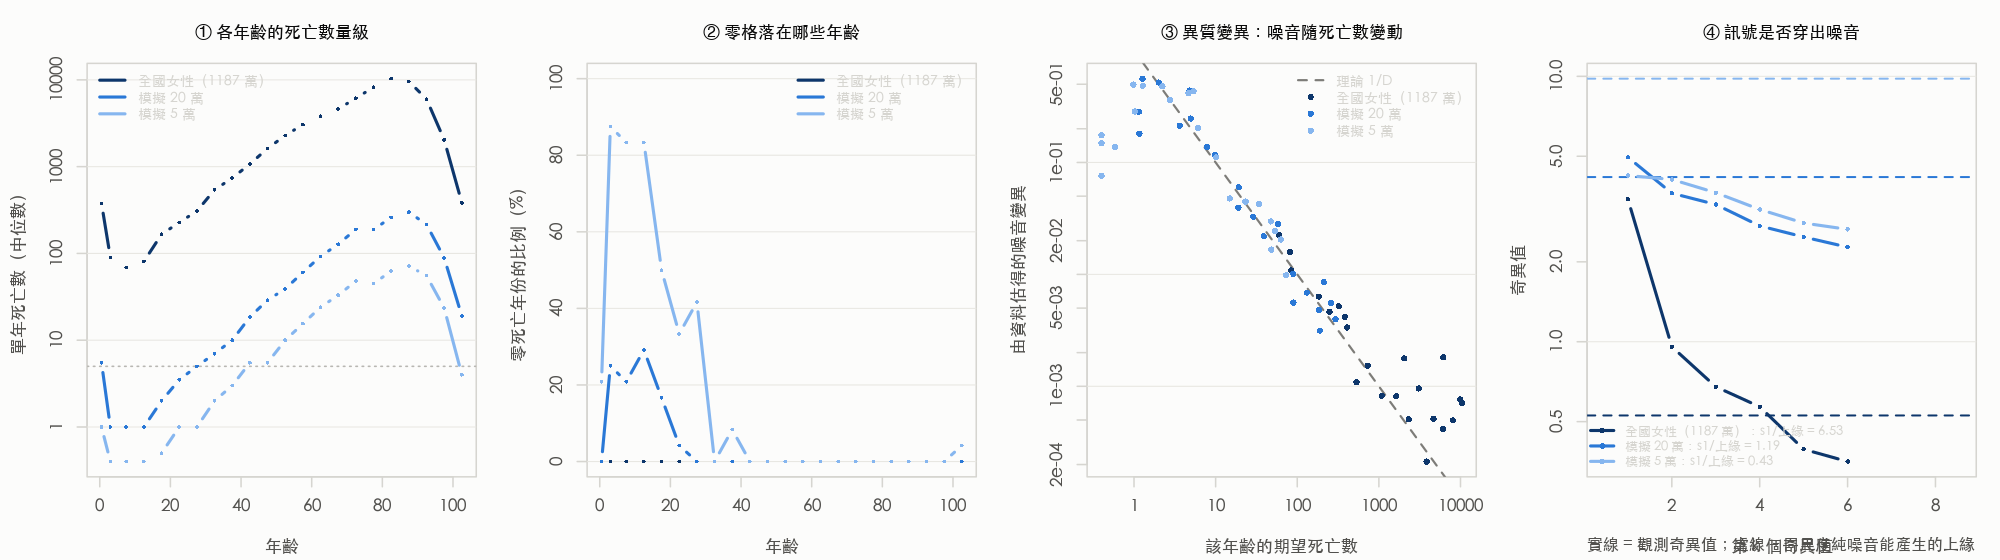
\includegraphics[width=\textwidth]{figEDA_panel.png}
  \caption{四項事前診斷。橫向比較全國女性實際資料與兩組模擬小人口
  （以全國配適為真值，$D_{x,t}\sim\mathrm{Poisson}(N w_x m^{\mathrm{true}}_{x,t})$）。
  \cn{1}\cn{2}\cn{3} 為純粹的探索性分析；\cn{4} 的噪音上緣需一次預備配適以估計 $\sigma$。}
  \label{fig:eda}
\end{figure}

\begin{table}[H]
  \centering
  \caption{四項診斷的數值摘要}
  \label{tab:eda}
  \small
  \begin{tabular}{lrrr}
    \toprule
    診斷項目 & 全國女性 & 模擬 20 萬 & 模擬 5 萬 \\
    \midrule
    \cn{1} 最小單年死亡數中位數        & 69   & 1     & 0     \\
    \cn{1} 死亡數的跨年齡落差（倍）    & 150  & 298   & 72    \\
    \cn{2} 零死亡格比例（\%）          & 0.0  & 4.4   & 18.8  \\
    \cn{2} 零格最集中的年齡組          & ---  & 10--14 & 1--4 \\
    \cn{3} 噪音變異的跨度（數量級）    & 2.0  & 2.3   & 1.7   \\
    \cn{4} 最大奇異值 $s_1$            & 3.44 & 4.96  & 4.23  \\
    \cn{4} 純噪音的上緣                & 0.53 & 4.17  & 9.80  \\
    \cn{4} $s_1\,/\,$上緣              & \textbf{6.53} & \textbf{1.19} & \textbf{0.43} \\
    \midrule
    判讀 & 訊號充分 & 邊緣 & 不可還原 \\
    \bottomrule
  \end{tabular}
\end{table}

\subsubsection{（一）計算方式}

\textbf{診斷\cn{1}} 取各年齡組單年死亡數的中位數，以對數刻度繪於年齡上。
須看兩件事：曲線的最低點是否進入個位數，以及最高與最低相差幾個數量級。

\textbf{診斷\cn{2}} 取各年齡組死亡數為零的年份比例。

\textbf{診斷\cn{3}} 以對數死亡率沿時間的二階差分估計噪音變異。二階差分消去
線性趨勢，而 $\mathrm{Var}(\Delta^2 X)=6\sigma^2$，故
$\widehat{\mathrm{Var}}=\mathrm{Var}(\Delta^2\log\hat m)/6$。以此對各年齡的
期望死亡數作雙對數散布圖，並加上理論參考線 $1/D$。

\textbf{診斷\cn{4}} 取中心化對數死亡率矩陣的奇異值譜，並加上純噪音所能產生的
上緣。依\S\ref{sec:bbp}，$n\times m$ 噪音矩陣的最大奇異值收斂至
$\sigma\sqrt{T}\,(1+\sqrt{c})$，$c=A/T$；而該文式 (9) 有一個便利的性質——
\textbf{在 BBP 相變門檻上，觀測到的最大奇異值恰好等於這條上緣}，故判讀
規則即為 $s_1$ 是否穿出虛線。

\subsubsection{（二）$\sigma$ 的估計方式會影響結論}

診斷\cn{4}需要 $\sigma$。本文比較三種事前可得的估法，並以已知結論
（$N\ge2\times10^5$ 可還原、$N=5\times10^4$ 邊緣、$N=10^4$ 不可還原）檢驗：

\begin{itemize}[leftmargin=*]
  \item \textbf{由觀測死亡數}：$\sigma=\sqrt{\overline{1/\max(D,0.5)}}$。
        可用但偏保守，若採用建議將門檻放寬至 1.2。
  \item \textbf{由預備配適的 $\hat\mu$}：$\sigma=\sqrt{\overline{1/\hat\mu}}$，
        其中 $\hat\mu$ 取自一次 Firth 卜瓦松配適，成本不到一秒。
        \textbf{本文採用此法}。
  \item \textbf{由二階差分}：\textbf{不可使用}。$N=10^4$ 時會誤判為可還原，
        因為四成零格被 0.5 墊平後，二階差分反映的是替代值的假象而非真噪音。
\end{itemize}

\subsubsection{（三）判讀門檻}

\begin{table}[H]
  \centering
  \caption{診斷\cn{4}的判讀門檻與對應建議}
  \label{tab:edarule}
  \small
  \begin{tabular}{llp{7.6cm}}
    \toprule
    $s_1/$上緣 & 判讀 & 建議 \\
    \midrule
    $>2$        & 訊號充分 & 各方法差異小，SVD 亦可 \\
    $1.2\sim2$  & 可還原   & 卜瓦松或加權 SVD（$w=\hat\mu$），加經驗貝氏收縮 \\
    $0.6\sim1.2$& 邊緣     & \textbf{方法選擇的效益最大}；卜瓦松／Firth 加收縮 \\
    $<0.6$      & 不可還原 & \textbf{不要以 SVD 估 $\beta_x$}；$\alpha_x$ 仍可靠 Firth 取得 \\
    \bottomrule
  \end{tabular}
\end{table}

須注意最後一列的措辭。BBP 門檻界定的是\textbf{未正則化的秩一分解}能還原
多少，並非所有估計量的上界；本文\S\ref{sec:est}顯示，
$N=5\times10^4$（比值 0.43）時標準 LC 的 $\hat\beta$ 與真值相關僅 0.037
（確實與隨機方向無異），但加上經驗貝氏收縮後可達 0.542。
\textbf{因此該格應讀為「不要用 SVD 估」，而非「無論如何都不能估」。}

\subsubsection{（四）診斷\cn{1}與 Wilmoth（1993）加權法的實務門檻}

綜合本文\S\ref{sec:est}的結果，診斷\cn{1}可給出兩個操作門檻：
最小單年死亡數中位數低於 5 時，Firth 為\textbf{必要}而非選配；
低於 20 時建議使用。死亡數的跨年齡落差超過一個數量級時，
等權重 SVD 已被誤設，應改用卜瓦松或以 $\hat\mu$ 加權的 SVD。

全國女性的 69 與 150 倍，即分別落在「安全」與「須加權」兩側——
\textbf{這說明即使在國家級資料上，加權仍是必要的}，只是零格的問題不存在。

\subsection{參數估計的偏誤診斷}\label{sec:diag}

老師於 2026 年 9 月 22 日的指導中指出：\textbf{應先由資料的分布特性與偏誤
特性出發，方能說明為何需要所提的方法}。本小節即依此要求，在進入任何
修勻或懲罰方法之前，先刻畫 LC 模型參數估計本身的行為。
圖示規格比照 Wang et al.（2018）第 354$\sim$355 頁。

\subsubsection{（一）設計與判讀方式}

以女性 2001$\sim$2024 年的 LC 配適為真值，令 $E_{x,t}=N\cdot w_{x,t}$、
$D_{x,t}\sim\text{Poisson}(E_{x,t}m^{\text{true}}_{x,t})$，
$N$ 取 $10^4$ 至 $5\times10^6$ 共九個水準，各重複 1{,}000 次。

除偏誤與標準誤外，本文另計算\textbf{T-ratio}：
\begin{equation}\label{eq:tratio}
T_x=\frac{\text{Bias}(\hat\theta_x)}{\mathrm{s.e.}(\hat\theta_x)} .
\end{equation}
其意義為\textbf{系統性偏誤相對於單次估計之抽樣標準差的倍數}。
$|T_x|>2$ 表示該年齡的偏誤已超過抽樣變異的兩倍，
亦即\textbf{偏誤}而非變異數才是該處的主要誤差來源；
反之 $|T_x|$ 很小則表示變異數主導。此一指標可直接回答
「究竟該先處理偏誤還是先處理變異數」。

\begin{figure}[H]
\centering
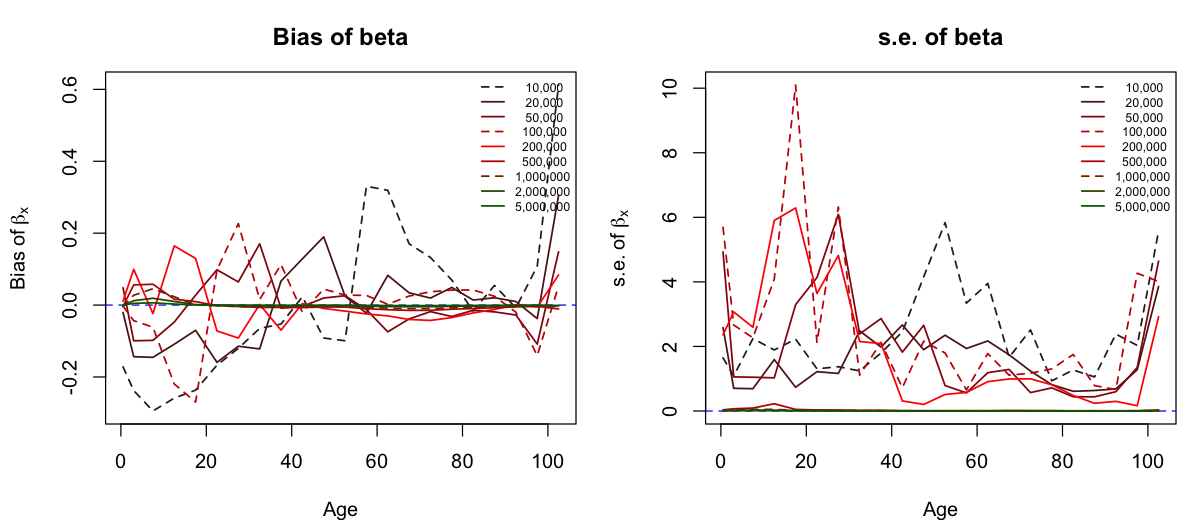
\includegraphics[width=\textwidth]{figE2_beta_bias_se.png}
\caption{$\hat\beta_x$ 的偏誤與標準誤（重複 1{,}000 次）。
左：偏誤；右：標準誤。曲線由深至淺對應人口規模 $10^4$ 至 $5\times10^6$。}
\label{fig:E2}
\end{figure}

\begin{figure}[H]
\centering
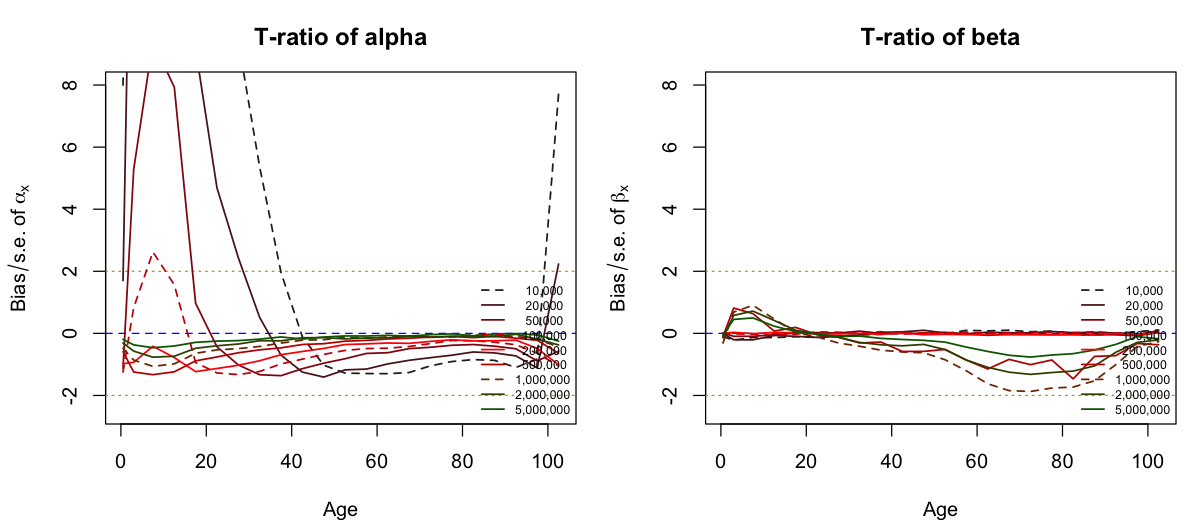
\includegraphics[width=\textwidth]{figE3_tratio.png}
\caption{$\hat\alpha_x$ 與 $\hat\beta_x$ 的 T-ratio。
虛線為 $\pm2$ 參考線；超出者表示偏誤大於兩倍抽樣標準差。}
\label{fig:E3}
\end{figure}

\subsubsection{（二）$\alpha_x$：小樣本下偏誤主導}

$\hat\alpha_x$ 的 T-ratio 在小樣本時極為可觀，且\textbf{集中於幼年組}：
$N=10^4$ 時 5$\sim$9 歲組達 \textbf{56.4}，$N=2\times10^4$ 時為 31.0，
$N=5\times10^4$ 時仍有 9.4，至 $N=10^5$ 降為 2.6，
$N\ge2\times10^5$ 後始全面落入 $\pm2$ 之內（表~\ref{tab:tratio}）。

\begin{table}[H]
\centering
\caption{各人口規模下 $|T|>2$ 的年齡組數與極值（共 22 組）}
\small
\begin{tabular}{rccrc}
\toprule
$N$ & $\alpha$ 之 $|T|>2$ 組數 & $\beta$ 之 $|T|>2$ 組數
 & $\alpha$ 之 $\max|T|$（年齡） & $\beta$ 之 $\max|T|$（年齡）\\
\midrule
$10^4$            & \textbf{9} & 0 & 56.4\ (5--9) & 0.22\ (1--4)\\
$2\times10^4$     & 7 & 0 & 31.0\ (5--9) & 0.21\ (5--9)\\
$5\times10^4$     & 3 & 0 & \phantom{0}9.4\ (5--9) & 0.09\ (1--4)\\
$10^5$            & 1 & 0 & \phantom{0}2.6\ (5--9) & 0.05\ (10--14)\\
$2\times10^5$     & 0 & 0 & \phantom{0}1.2\ (15--19) & 0.05\ (85--89)\\
$5\times10^5$     & 0 & 0 & \phantom{0}1.3\ (5--9) & \textbf{1.47}\ (80--84)\\
$10^6$            & 0 & 0 & \phantom{0}1.1\ (5--9) & \textbf{1.87}\ (70--74)\\
$2\times10^6$     & 0 & 0 & \phantom{0}0.8\ (5--9) & 1.32\ (70--74)\\
$5\times10^6$     & 0 & 0 & \phantom{0}0.5\ (5--9) & 0.76\ (70--74)\\
\bottomrule
\end{tabular}
\label{tab:tratio}
\end{table}

此一型態與 Wang et al.（2018）及老師 2026 年 9 月的簡報所述
「$\alpha_x$ 的偏誤最為顯著」完全一致。偏誤集中於幼年組的原因見
表~\ref{tab:datadesc}：5$\sim$9 歲組的單年死亡數中位數僅 69 人，
在 $N=10^4$ 的情境下期望死亡數不足 1，零格與對數轉換的影響於此最為劇烈。

\subsubsection{（三）$\beta_x$：T-ratio 的非單調型態}\label{sec:betaT}

$\hat\beta_x$ 的情形\textbf{與 $\alpha_x$ 截然不同，且出乎意料}。
其 T-ratio 在小樣本時\textbf{極小}（$N\le2\times10^5$ 時 $\max|T|<0.25$），
隨 $N$ 增大反而\textbf{上升}至 $N=10^6$ 的 1.87（70$\sim$74 歲組），
其後又下降至 $5\times10^6$ 的 0.76——呈現明顯的\textbf{非單調}型態。

\textbf{此一型態不可誤讀。} 小樣本時 $|T|$ 接近零，\textbf{並不代表
$\hat\beta_x$ 估得好}，而是其抽樣標準差大到使偏誤相形之下微不足道：
$N=10^4$ 時 $\hat\beta_x$ 與真值的相關中位數為 $-0.24$，
估計值實質上已無資訊。換言之，
\textbf{小樣本下 $\beta_x$ 的問題是變異數，不是偏誤}。
待 $N$ 增至 $5\times10^5$ 以上、變異數收斂之後，
原先被掩蓋的偏誤才浮現為顯著（60$\sim$90 歲組的 $|T|$ 接近 2），
此時\textbf{偏誤才成為誤差的主要成分}。

\subsubsection{（四）本小節對研究設計的意涵}

\textbf{$\alpha_x$ 與 $\beta_x$ 的病因並不相同，因而不應以同一種方法處理。}

\begin{itemize}
  \item $\alpha_x$：小樣本下\textbf{偏誤}主導（$N\le10^5$ 時 $|T|$ 可達 56），
        須以\textbf{校正偏誤}的手段處理。
  \item $\beta_x$：小樣本下\textbf{變異數}主導，
        \textbf{收縮類方法（含本文的懲罰項）於此有其正當性}；
        惟 $N\ge5\times10^5$ 後偏誤轉為主要成分，
        此時固定強度的收縮反而有害——此即第柒節之六所觀察到的
        「固定比例的懲罰在 $N\ge3\times10^5$ 後反受其害」的成因。
\end{itemize}

\noindent\textbf{此一區分修正了本文早期版本的論述。} 先前將
「小樣本的問題是偏誤而非變異數」作為通則陳述，
現依 T-ratio 的證據應修正為：\textbf{$\alpha_x$ 與漂移項是偏誤問題，
$\beta_x$ 在小樣本是變異數問題、在大樣本才轉為偏誤問題}。
此一修正亦與 Wang et al.（2018）與老師簡報中
「Partial SMR 對 $\alpha_x$ 的偏誤有顯著改善、對 $\beta_x$ 則改善有限」
的結果相互印證。

\subsection{比較的六種方法}

本文比較六種 LC 變體，如表~\ref{tab:variants} 所示。其中 LC、LCP、LM、BMS 為對照組，
$\LCe$ 為 Rabbi and Mazzuco（2021）的還原對象，M$\LCe$ 則為本文額外設計
的變體——先以修勻後的期望死亡數走卜瓦松最大概似，再對齊 $\edag$，用以分離
「修勻」與「卜瓦松架構」兩項效果。

\begin{table}[H]
\centering
\caption{本文比較的六種 Lee-Carter 變體}
\small
\begin{tabular}{llll}
\toprule
簡稱 & 修勻 & 估計架構 & $\kappa_t$ 的調整方式\\
\midrule
LC      & 無 & SVD & 對齊總死亡數\\
LCP     & 無 & 卜瓦松 MLE & 不需調整\\
LM      & 無 & SVD & 對齊 $e_0$\\
BMS     & 無 & 卜瓦松 MLE & 另搜尋最適配適起始年\\
$\LCe$  & 二維 $L_1$ & SVD & 對齊 $\edag$\\
M$\LCe$ & 二維 $L_1$ & 卜瓦松 MLE & 對齊 $\edag$\\
\bottomrule
\end{tabular}
\label{tab:variants}
\end{table}

\subsection{電腦模擬設計}

本文以女性 2001$\sim$2024 年的 LC 配適結果作為真值
$(\alpha_x,\beta_x,\kappa_t)$，令暴露數 $E_{x,t}=N\cdot w_{x,t}$，其中
$w_{x,t}$ 為各年的年齡結構（各年合計為 1），$N$ 為單一性別總人數；死亡數則
由 $D_{x,t}\sim\text{Poisson}(E_{x,t}\,m^{\text{true}}_{x,t})$ 產生。$N$ 的
範圍取 1 萬至 100 萬，涵蓋我國絕大多數鄉鎮市區與縣市的規模。

\section{論文還原結果}

\subsection{成立的部分}

\subsubsection{（一）LASSO 修勻的配適精確度優於樣條函數方法}

表~\ref{tab:smooth} 呈現三種修勻法在女性 2001$\sim$2024 年資料上的配適誤差
與粗糙度，用以回應\textbf{問題一的第一個環節}：原文宣稱 LASSO 型修勻優於
樣條，此一宣稱在臺灣資料上是否重現。為使比較乾淨，本文以同一組差分算子的
$L_2$ 版本作為樣條的對照，使三種方法\textbf{僅差在所用的 norm}，
而非同時差在差分算子與 norm 兩處。

表中四個指標的意義如下。MAE 與 MSE 衡量\textbf{修勻後的曲面與觀測值的
距離}，數值越小代表越貼近資料；年齡方向與時間方向的粗糙度則以二階差分的
平均絕對值衡量\textbf{曲面本身的起伏}，數值越小代表越平滑。兩類指標方向
相反：修勻必然以增加前者換取減少後者，因此\textbf{單看任一類指標都無法
判定優劣}。

觀察結果，LASSO 的 MAE（0.0413）與 MSE（0.0047）均為三者最小，
時間方向粗糙度（0.0012）亦最小，但\textbf{年齡方向粗糙度（0.0179）反而
高於}兩種 $L_2$ 樣條（0.0137 與 0.0140）。這與原文所述
「較不平滑但誤差較小」的性質吻合：$L_1$ norm 容許曲面在少數年齡保留
轉折，以換取整體誤差的下降，而 $L_2$ norm 則把起伏均勻地攤平到所有年齡。

此一結果\textbf{支持原文的宣稱}，但也顯示該宣稱的成立僅限於「配適精確度」
這一面向。修勻的最終目的並非貼近觀測值，而是改善後續的參數估計與預測，
因此\textbf{配適精確度較佳並不保證下游表現較佳}。本文接續以樣本外評估
（第伍節之二）與預測區間（第伍節之三）檢驗此一推論鏈的後半段。

\begin{table}[H]
\centering
\caption{三種修勻法的比較（女性 2001$\sim$2024 年）}
\small
\begin{tabular}{lcccc}
\toprule
修勻法 & MAE & MSE & 年齡方向粗糙度 & 時間方向粗糙度\\
\midrule
觀測值 & --- & --- & 0.0204 & 0.0981\\
一維樣條（$L_2$，年齡） & 0.0538 & 0.0218 & 0.0140 & 0.0908\\
二維樣條（$L_2$） & 0.0759 & 0.0247 & \textbf{0.0137} & 0.0025\\
LASSO（$L_1$） & \textbf{0.0413} & \textbf{0.0047} & 0.0179 & \textbf{0.0012}\\
\bottomrule
\end{tabular}
\label{tab:smooth}
\end{table}

\begin{figure}[H]
\centering
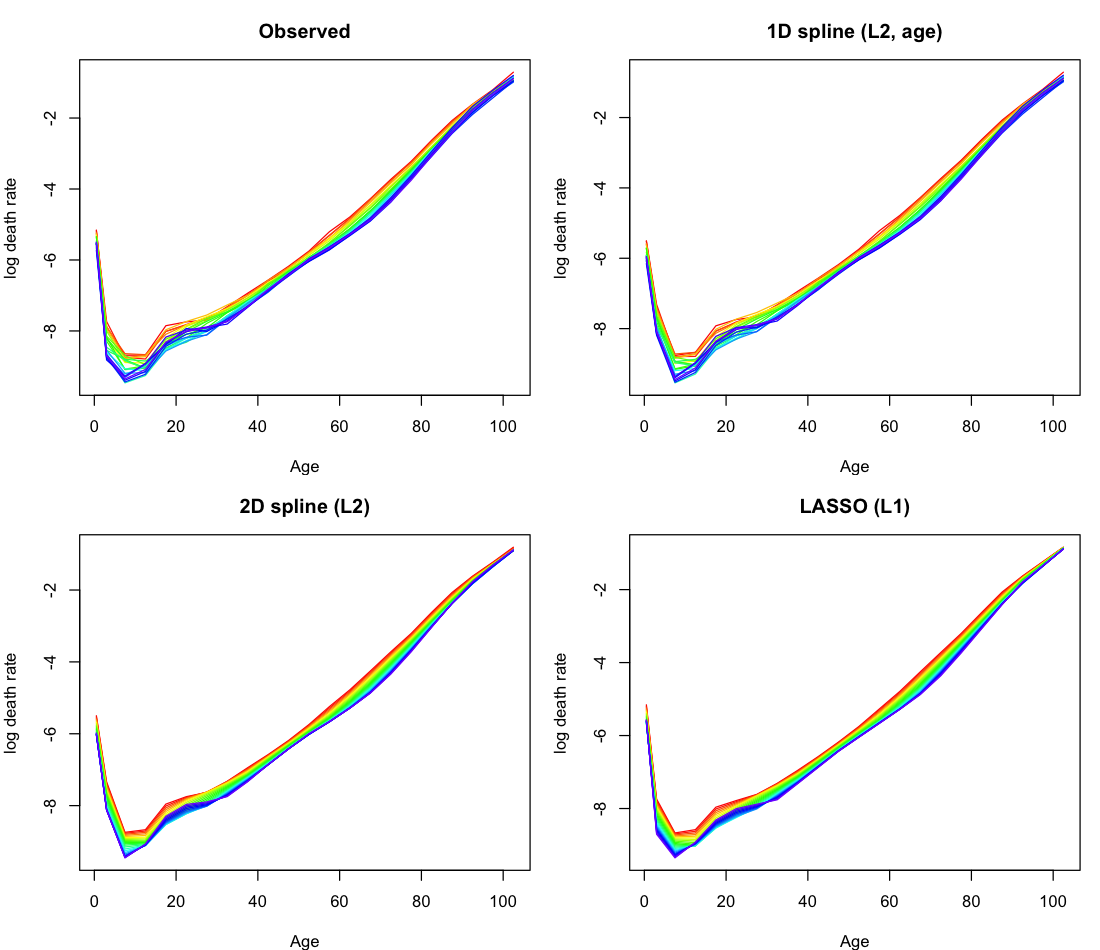
\includegraphics[width=0.82\textwidth]{fig1_smoothing.png}
\caption{三種修勻法的死亡率曲面（女性 2001$\sim$2024 年，每條線為一年）}
\label{fig:smooth}
\end{figure}

\subsubsection{（二）$e_0$ 與 $\edag$ 的反向關係成立}

女性 2001$\sim$2024 年，$e_0$ 由 79.64 歲升至 83.94 歲，$\edag$ 由 11.76
降至 10.85，相關係數為 $-0.944$，與原文所述一致。

\subsubsection{（三）$\edag$ 調整使 $\kappa_t$ 更接近線性}

如表~\ref{tab:kappa}，離線性殘差標準差由 LC 的 0.960 降至 $\LCe$ 的 0.726 與 M$\LCe$ 的
0.703，該文的核心主張在此配適期成立。

\begin{table}[H]
\centering
\caption{六種方法的 $\kappa_t$ 性質（女性 2001$\sim$2024 年）}
\small
\begin{tabular}{lccc}
\toprule
方法 & 漂移項 & $\sigma$（一階差標準差） & 離線性殘差標準差\\
\midrule
LC      & $-0.4126$ & 0.8505 & 0.9598\\
LCP     & $-0.4091$ & 0.6799 & 0.7971\\
LM      & $-0.4064$ & 0.7318 & 0.9071\\
BMS     & $-0.4042$ & 0.6895 & 0.7864\\
$\LCe$  & $-0.3593$ & 0.8794 & 0.7262\\
M$\LCe$ & $-0.3491$ & 0.8566 & \textbf{0.7026}\\
\bottomrule
\end{tabular}
\label{tab:kappa}
\end{table}

\subsection{不成立或需要限定的部分}

\subsubsection{（一）優勢僅限於近期短配適期}\label{sec:window}

表~\ref{tab:panel} 呈現「性別 $\times$ 配適起始年」共 12 格面板的樣本外
平均絕對誤差，用以回應\textbf{問題一的核心}：前述在單一設定下成立的優勢，
是否為普遍的性質。若僅看女性 2001 年起算、留最後 5 年的結果，$\LCe$ 在四個
指標上同時最佳，這是原文主張最強的證據；\textbf{本文的假說是，若該方法確實
較優，則此一優勢應在不同性別與不同配適期上一致重現}。

表中的指標為樣本外的平均絕對誤差，數值越小代表預測越準；每列以粗體標示該格
的最佳方法。因此\textbf{只需觀察粗體落在哪一欄，即可判定優勢是否普遍}。

觀察結果，$\LCe$ 與 M$\LCe$ 僅在 2001、1991 年起算的 5 格勝出，
其餘 7 格全部由 LM 奪冠，且 1981、1971 年起算的長配適期\textbf{無一例外}。
\textbf{此與前述假說不吻合}：優勢並非普遍存在，而是\textbf{隨配適期拉長而
系統性消失}。

\begin{table}[H]
\centering
\caption{各面板格的樣本外 MAE（$h=5$）；粗體為該格最佳}
\small
\begin{tabular}{lcccc@{\hspace{14pt}}lcccc}
\toprule
起始年 & $\LCe$ & M$\LCe$ & LM & LC & 起始年 & $\LCe$ & M$\LCe$ & LM & LC\\
\midrule
女 2001 & \textbf{.0962} & \textbf{.0962} & .1080 & .1194 & 男 1981 & .1323 & --- & \textbf{.1099} & .1454\\
女 1991 & .0992 & \textbf{.0988} & .1064 & .1197 & 男 1971 & .1124 & --- & \textbf{.1078} & .1353\\
女 1981 & .1194 & .1202 & \textbf{.1057} & .1163 & 總 2001 & .0862 & \textbf{.0841} & .0967 & .1141\\
女 1971 & .1172 & .1152 & \textbf{.1061} & .1300 & 總 1991 & .0945 & \textbf{.0905} & .0956 & .1266\\
男 2001 & .0965 & \textbf{.0942} & .1062 & .1232 & 總 1981 & .1080 & --- & \textbf{.0950} & .1268\\
男 1991 & .1243 & --- & \textbf{.1090} & .1436 & 總 1971 & .1005 & --- & \textbf{.0935} & .1227\\
\bottomrule
\end{tabular}
\label{tab:panel}
\end{table}

同一套程式套用於全人口 1970$\sim$2024 年時，$\edag$ 調整反而使 $\kappa_t$
\textbf{更不線性}（離線性殘差標準差 1.824，原始 LC 僅 0.848），方向與主分析
配適期完全相反。兩項證據指向同一結論：\textbf{該方法的優勢是配適期的函數，
而非方法本身的固有性質}。原文的 20 個國家全部採用 1950 年起的長序列，
並未檢驗配適期的敏感度，因而無從發現此一限制；這與 Basellini et al.（2023）
強調「配適期的選擇對預測影響重大、卻常被略過說明」的論點完全吻合。

此一現象提出了一個本節無法回答的問題：\textbf{配適期之所以重要，
究竟是因為它改變了可用的資訊量，還是因為長配適期違反了 $\beta_x$ 不隨時間
變動的假設？} 兩者的補救方式完全不同——前者只需更多資料，後者則須修改
模型。由於在實際資料上配適期與資料量必然同時變動，無法分離，
本文於\S\ref{sec:TN} 另行設計「配適期長度 $\times$ 人口規模」的二因子模擬，
以固定其一、變動其二的方式回應此一問題。

\subsubsection{（二）預測區間不是更窄而是更寬}

原文將「$\kappa_t$ 更線性」與「區間更窄」綁在一起論述，但兩者並不等價。
如表~\ref{tab:e0}，$\LCe$ 的 $\kappa_t$ 一階差標準差為 0.879，反而略高於 LC 的 0.851，
因此其 2050 年 $e_0$ 的 80\% 預測區間寬度 3.977 為六種方法中最寬者。

\begin{table}[H]
\centering
\caption{2050 年女性零歲平均餘命的預測與 80\% 預測區間}
\small
\begin{tabular}{lccc}
\toprule
方法 & $e_0$（2050） & 80\% 預測區間 & 區間寬度\\
\midrule
LC      & 87.99 & $[86.10,\ 89.69]$ & 3.591\\
LCP     & 88.02 & $[86.53,\ 89.40]$ & \textbf{2.875}\\
LM      & 87.86 & $[86.25,\ 89.34]$ & 3.090\\
BMS     & 87.95 & $[86.45,\ 89.34]$ & 2.895\\
$\LCe$  & 87.61 & $[85.51,\ 89.49]$ & \textbf{3.977}\\
M$\LCe$ & 87.47 & $[85.45,\ 89.29]$ & 3.842\\
\bottomrule
\end{tabular}
\label{tab:e0}
\end{table}

\subsubsection{（三）涵蓋率的優勢是建立在寬度的犧牲之上}

$\LCe$ 的涵蓋機率偏差雖為六者最低（0.20），但平均區間寬度 1.391 是 LC 的
0.875 的 1.6 倍。更重要的是，六種方法的實證涵蓋率都落在 0.2$\sim$0.6 之間，
距名目的 0.8 甚遠。「LC 模型的預測區間過窄」此一診斷最早由 Alho（1992）在對原文的評論中提出，
其後 Shang et al.（2011）以更大規模的比較加以確認。本文的結果與其方向一致——
Shang et al.（2011）比較 10 種 LC 擴充、
14 個國家後得到「全部低估死亡率變異性」的結論一致，惟本文係在單一人口、
五齡組、且留出期涵蓋 COVID-19 的條件下取得，程度嚴重得多。

\subsection{論文還原過程浮現的方法論問題}

\textbf{（一）原文圖 8 的相關係數受模型結構決定，其論證不一定成立。}
觀測值的 $e_0$ 與 $\edag$ 相關係數為 $-0.944$，配適值則高達 $-0.999$。由於
秩 1 的 LC 模型中每年的整條死亡率曲線由單一純量 $\kappa_t$ 決定，$e_0$ 與
$\edag$ 必然都是 $\kappa_t$ 的單調函數，因而近乎完美相關。此一數值僅說明
模型已丟棄所有橫斷面變異，原文據以比較相關係數高低的論證並不成立。

\textbf{（二）$\edag$ 對 $\kappa$ 是單峰而非單調。}
本文計算發現，$\edag(\kappa)$ 由 $\kappa=-80$ 的約 6 升至 $\kappa\approx54$
的峰值 30.2，再降至 $\kappa=+80$ 的 2.4。此一形狀在人口學上合理：死亡率極高
時死亡集中於幼年、極低時集中於高齡，兩端的死亡年齡差異皆小。其後果是
「以 $\edag$ 對齊 $\kappa_t$」原則上可能存在兩個解。低死亡率國家的 $\kappa_t$
離峰頂甚遠，實務上不致遭遇，但高死亡率人口或極端外推情境未必如此。原文對此
前提並未討論，本文的實作因此改以網格掃描取最接近原值的根。

\textbf{（三）原文選取修勻參數的準則在台灣數據上傾向選擇「不修勻」。}
該文以對觀測值的 MAE 與 MSE 比較各種修勻法，而修勻依定義必然增加對觀測值
的誤差。本文以留出格重算此一準則，在 $N=5$ 萬與 20 萬時，最小值均落在
$\lambda=0$。此非方法優劣的比較，而是準則的定義使然。

\section{偏誤來源與估計量的選擇}

\subsection{暴露數對估計的影響}

本小節回應\textbf{問題二}：小樣本下 LC 模型失效的機制，究竟是變異數增大
還是有方向的偏誤。實際資料無從分辨此二者，因為真值未知；本文因此以蒙地
卡羅模擬建立一個\textbf{已知真值}的環境，固定年齡結構與死亡率型態、
僅變動人口規模 $N$，觀察估計量隨 $N$ 的變化。

表~\ref{tab:mc} 與圖~\ref{fig:mc} 呈現四項指標。\textbf{零死亡格數}衡量
資料的稀疏程度，數值越大表示越多年齡年份組合無死亡發生；
\textbf{$\alpha_x$ 的平均偏誤}若顯著偏離零，即為有方向的偏誤而非隨機誤差；
\textbf{$\beta_x$ 相關中位數}衡量年齡型態的還原程度，接近 1 表示形狀正確、
接近 0 或為負則表示估計結果與真實型態無關；\textbf{漂移項中位數}應與真值
$-0.3678$ 比較，偏向零即代表低估死亡改善速度。

\textbf{本文的假說是}：若失效只是變異數問題，則各項指標應\textbf{環繞真值
對稱散布}，僅離散程度隨 $N$ 減小而擴大；若存在偏誤，則指標的\textbf{中位數
本身}會系統性偏離真值。

\begin{table}[H]
\centering
\caption{暴露數對 Lee-Carter 模型估計的影響（重複 100 次；漂移項真值 $-0.3678$）}
\small
\begin{tabular}{rcccc}
\toprule
$N$ & 零死亡格數／528 & $\alpha_x$ 平均偏誤 & $\beta_x$ 相關中位數（LC／LASSO） & 漂移項中位數\\
\midrule
10,000    & 214.0 & $\mathbf{+0.439}$ & $-0.240$／$-0.441$ & $-0.110$\\
50,000    & 89.2  & $+0.033$ & $-0.045$／$+0.045$ & $-0.065$\\
200,000   & 21.7  & $-0.051$ & $+0.564$／$+0.552$ & $-0.216$\\
1,000,000 & 0.3   & $-0.021$ & $+0.823$／$+0.862$ & $-0.340$\\
\bottomrule
\end{tabular}
\label{tab:mc}
\end{table}

\begin{figure}[H]
\centering

\includegraphics[width=0.80\textwidth]{mc_plots.png}
\caption{暴露數與估計方法的蒙地卡羅模擬結果}
\label{fig:mc}
\end{figure}

觀察結果，\textbf{與「純變異數」的假說明顯不吻合}：$\alpha_x$ 的平均偏誤
在 $N=1$ 萬時高達 $+0.439$，方向一致為正；漂移項中位數在所有 $N$ 下
\textbf{一律偏向零}（$-0.110$ 至 $-0.340$，真值 $-0.3678$），從未出現高估。
兩者都是\textbf{系統性的方向偏移}，而非對稱的隨機散布。

\textbf{惟此一結論須依參數分別陳述}（詳見\S\ref{sec:diag} 的 T-ratio 診斷）：
$\alpha_x$ 與漂移項確為\textbf{偏誤}問題——$\alpha_x$ 在 $N\le10^5$ 時
$|T|$ 可達 56，漂移項在所有 $N$ 下一律偏向零；
而 $\beta_x$ 在小樣本時 $|T|<0.25$，其誤差\textbf{由變異數主導}，
須至 $N\ge5\times10^5$ 變異數收斂後，偏誤才成為主要成分。
此一區分之所以重要，在於兩者的補救方式完全相反——變異數問題可藉由收縮
（即本文第柒節的懲罰項）處理，偏誤則必須找出來源並加以校正，
加寬區間或增加重複皆無濟於事。

以下分述四項發現。

\textbf{其一，$N\le2$ 萬時零死亡格佔四成，主導估計品質的是零格處理而非估計
方法。} $\alpha_x$ 的正向偏誤 $+0.439$ 即來自期望死亡數低於 0.5 的格子被
墊高，修勻參數 $\lambda$ 由 0 增至 20 均無法改善（偏誤始終在 0.38 至 0.45
之間）。此一結果與 Wang et al.（2018）、余清祥等（2021）發現
「$\alpha_x$ 的偏誤較 $\beta_x$ 更為嚴重」完全一致，本文並進一步指出其成因。
值得一提的是，Wilmoth（1993）建議的「給零格零權重」經本文測試後發現反而
更差（$N=20$ 萬時 $\beta_x$ 相關降至 0.11），因為捨棄零格等於捨棄
「此處死亡率很低」的訊息。

\textbf{其二，$N\le20$ 萬時兩種方法的 $\beta_x$ 都已崩潰}，須至 100 萬人年
才有 0.82（LC）至 0.86（LASSO）的相關。此一門檻與王信忠等（2012）建議「小區域人數小於 20 萬時
需特別謹慎」相符。（本文並確認估計流程無誤：$N=10^8$ 時相關為 0.999。）

\textbf{其三，漂移項被系統性壓平，小人口低估死亡改善速度。} 這是有方向的
偏誤，較變異數增大更為嚴重，因為漂移項直接乘上預測期長度進入平均餘命。

\textbf{其四，LASSO 修勻最明確的貢獻是把漂移項拉回真值附近並使四分位距
減半}（$N\ge5$ 萬時），而非降低 $\beta_x$ 的變異。

\vspace{4pt}
上述結果把問題二推進了一步，卻也留下兩個待答的環節。
\textbf{其一，偏誤的來源為何？} 若來自零格處理，則改變零格的處理方式應可
改善；若來自對數轉換本身，則須改換估計架構。本文於\S\ref{sec:decomp} 以
「卜瓦松最大概似取代 SVD」的對照實驗分離此二者——\textbf{卜瓦松架構不取
對數、亦不需替代零格}，若偏誤在該架構下消失，即可歸因於對數轉換。
\textbf{其二，偏誤如何傳導到預測區間？} 偏誤使區間\textbf{擺錯位置}、
變異數使區間\textbf{寬度不當}，兩者對涵蓋率的影響可能相互抵銷而不易分辨。
本文於\S\ref{sec:isrc} 設計四個層層疊加的區間變體（僅未來創新、插入式、
加計參數不確定性、加計修勻），\textbf{以逐項加入的方式辨識各成分的貢獻}。

\subsection{修勻參數的選擇}

四種選法與「已知真值」的 oracle 對照如表~\ref{tab:lamsel}。交叉驗證在大人口
能準確命中最適 $\lambda$（相對損失 1.07），但在小人口則修勻不足、相對損失
達 3.5 倍。其原因並非交叉驗證失效，而是交叉驗證衡量的是「曲面」的預測誤差，
而 $\beta_x$ 是曲面的泛函（Functional）、對雜訊敏感得多，兩者所需的修勻程度
不同，且落差在最需要修勻的小人口最大。

\begin{table}[H]
\centering
\caption{$\lambda$ 各種選法與 oracle 的對照（重複 100 次）}
\small
\begin{tabular}{rcccccc}
\toprule
& \multicolumn{2}{c}{oracle} & \multicolumn{2}{c}{交叉驗證}
& \multicolumn{2}{c}{參數式拔靴}\\
\cmidrule(lr){2-3}\cmidrule(lr){4-5}\cmidrule(lr){6-7}
$N$ & $\lambda$ & SSE($\beta$) & SSE($\beta$) & 相對損失
    & SSE($\beta$) & 相對損失\\
\midrule
50,000    & 40 & 0.0253 & 0.0881 & 3.49 & 0.0531 & \textbf{2.10}\\
200,000   & 20 & 0.0062 & 0.0175 & 2.82 & 0.0065 & \textbf{1.05}\\
1,000,000 & \phantom{0}5 & 0.0036 & 0.0038 & \textbf{1.07} & 0.0039 & 1.09\\
\bottomrule
\end{tabular}
\label{tab:lamsel}
\end{table}
此外，$\lambda=0$ 根本無法被交叉驗證——沒有修勻
就無法對留出格產生預測——因此該準則回答不了「要不要修勻」。

本文改採\textbf{參數式拔靴法的插入式選法}（直接瞄準 $\hat\beta_x$ 的誤差
平方和），在小人口明顯較佳（相對損失 2.10 對交叉驗證的 3.49），
在 $N=20$ 萬時更幾乎追平 oracle（1.05）。Delwarde et al.（2007）的平滑參數亦以交叉驗證選取，
本文的結果顯示該準則在小人口會系統性偏誤，可作為該方法的直接補充。

\subsection{三個方向的修勻參數應分開設定}

原文以單一 $\lambda$ 連動三個方向，本文將其拆開後發現（表~\ref{tab:lam3}），交叉項
$\lambda_{xt}$ 才是主力：兩個暴露數的前八名全部 $\lambda_{xt}>0$，最差三名
全部 $\lambda_{xt}=0$，純年齡方向的修勻甚至比完全不修勻更糟。其原因可由
LC 模型的結構直接推得：
\begin{equation}
\frac{\partial^2\log m_{x,t}}{\partial x\,\partial t}=\beta'_x\,\kappa'_t,
\end{equation}
亦即交叉項本質上就是對 $\beta_x$ 粗糙度的懲罰，是三個方向中唯一直接瞄準
$\beta_x$ 者。此點在數學上與 Delwarde et al.（2007）的估計中修勻等價，惟
作用於曲面而非參數。

\begin{table}[H]
\centering
\caption{三方向修勻參數的格點搜尋（$N=20$ 萬，重複 100 次）}
\small
\begin{tabular}{ccccc l}
\toprule
$\lambda_{xx}$ & $\lambda_{xt}$ & $\lambda_{tt}$ & SSE($\beta$) & SSE($\alpha$) & 說明\\
\midrule
20 & 5 & 5  & \textbf{0.0054} & 4.380 & $\beta$ 最佳但 $\alpha$ 崩壞\\
20 & 5 & 20 & 0.0056 & 4.432 & \\
20 & 5 & 1  & 0.0059 & 4.476 & \\
1  & 5 & 5  & 0.0072 & \textbf{0.196} & 兼顧兩者的選擇\\
0  & 0 & 0  & 0.0540 & 0.224 & 不修勻\\
20 & 0 & 0  & 0.1135 & 6.157 & 比不修勻更糟\\
\bottomrule
\end{tabular}
\label{tab:lam3}
\end{table}

\subsection{配適期長度與人口規模的二因子設計}\label{sec:TN}

本小節回應第伍節之二留下的問題：配適期之所以重要，是因為它改變了可用的
資訊量，還是因為長配適期違反了 $\beta_x$ 不隨時間變動的假設。在實際資料上
配適期一拉長、可用資料量必然同時增加，兩者無法分離；\textbf{模擬的價值
正在於可以固定其一、只變動其二}。

\textbf{三種情境的預期形貌}：若\textbf{（甲）只有資訊量重要}，則 $T$ 與 $N$
可互相替代，任何 $(T,N)$ 只要乘積相近、表現就應相近；
若\textbf{（乙）$\beta_x$ 的穩定性是主要限制}，則拉長 $T$ 反而會因納入過時
的年齡型態而使表現變差；
若\textbf{（丙）$T$ 另有獨立於資訊量的作用}，則增加 $N$ 無法補償 $T$ 的
不足，表現會在某個 $T$ 以下出現無法以人口規模跨越的下限。
\textbf{三種情境在結果表上的形貌截然不同，因而可據以區辨}。

本小節因此以 $T\times N$ 的二因子設計分離兩個脆弱來源：以女性
1970$\sim$2024 年（55 年）的配適為真值，對每個 $(T,N)$ 組合模擬最近 $T$ 年的
死亡數並重新估計，$T\in\{10,15,20,30,40,55\}$、$N\in\{2\times10^4, 5\times10^4,
2\times10^5, 10^6\}$，各重複 100 次。

\textbf{評估指標改用 $\hat\beta_x$ 與真值的相關係數，而非誤差平方和。}
原因是在 $T$ 與 $N$ 都很小時，$\kappa_t$ 的變化範圍不足以識別 $\beta_x$，
估計值會\textbf{完全退化為均勻向量} $\mathbf{1}/A$；此時誤差平方和恰為
$\|\mathbf{1}/A-\beta^{\text{true}}\|^2=0.0070$，反而\textbf{小於}
$T$ 稍長但估計值劇烈震盪時的數值，若只看誤差平方和會誤判為「短配適期較佳」。
表~\ref{tab:TNdegen} 的退化率即為此現象的直接證據。

\begin{table}[H]
\centering
\caption{$\hat\beta_x$ 與真值的相關係數中位數（未懲罰，重複 100 次）}
\small
\begin{tabular}{rcccc}
\toprule
$T$（年） & $N=2\times10^4$ & $N=5\times10^4$ & $N=2\times10^5$ & $N=10^6$\\
\midrule
10 & 0.247 & 0.156 & 0.170 & 0.120\\
15 & 0.188 & 0.191 & 0.226 & 0.465\\
20 & 0.178 & 0.217 & 0.407 & 0.760\\
30 & 0.323 & 0.593 & 0.785 & \textbf{0.952}\\
40 & 0.508 & 0.725 & \textbf{0.899} & \textbf{0.977}\\
55 & 0.746 & \textbf{0.874} & \textbf{0.966} & \textbf{0.991}\\
\bottomrule
\end{tabular}
\label{tab:TNcor}
\end{table}

\begin{table}[H]
\centering
\caption{退化率：$\hat\beta_x$ 完全塌陷為 $\mathbf{1}/A$ 的比例}
\small
\begin{tabular}{rcccc}
\toprule
$T$（年） & $N=2\times10^4$ & $N=5\times10^4$ & $N=2\times10^5$ & $N=10^6$\\
\midrule
10 & \textbf{0.81} & 0.27 & 0 & 0\\
15 & \textbf{0.53} & 0.04 & 0 & 0\\
20 & 0.22 & 0 & 0 & 0\\
$\ge30$ & 0 & 0 & 0 & 0\\
\bottomrule
\end{tabular}
\label{tab:TNdegen}
\end{table}

\begin{figure}[H]
\centering
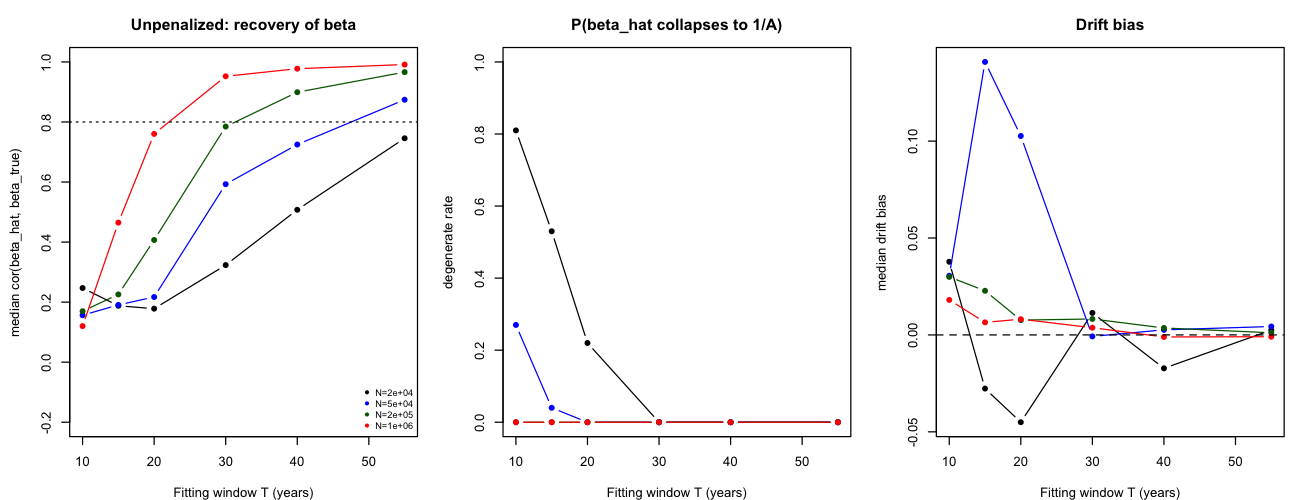
\includegraphics[width=\textwidth]{figB_TxN.png}
\caption{配適期長度 $T$ 與人口規模 $N$ 的二因子結果。虛線為相關係數 0.8。}
\label{fig:TN}
\end{figure}

\textbf{結果落在情境（丙）}。若情境（甲）成立，$T=10$、$N=10^6$
（資訊量與 $T=55$、$N\approx2\times10^5$ 相當）的表現應與後者接近，
但實際上前者僅 0.120、後者達 0.966，相差近八倍；情境（乙）亦不成立，
因為拉長 $T$ 在所有 $N$ 下都使表現\textbf{單調變好}，未見過時年齡型態
造成的反轉。\textbf{亦即 $T$ 具有獨立於資訊量的作用}。以下分述三項發現。

\textbf{其一，配適期長度比人口規模更關鍵。} 在 $T=10$ 年時，即使人口達
$10^6$，相關係數僅 0.120，幾乎完全無法還原 $\beta_x$；反之在 $T=55$ 年時，
即使人口僅 $2\times10^4$ 也能達到 0.746。
\textbf{「長配適期配小人口」明顯優於「短配適期配大人口」}，
這是單看 $N$ 的模擬設計無法得到的結論。

\textbf{其二，兩者存在等準確度的替換關係。} 以相關係數 0.8 為可用門檻，
$T=55$ 年需 $N\ge5\times10^4$、$T=40$ 年需 $N\ge2\times10^5$、
$T=30$ 年需 $N\ge10^6$；而 $T\le20$ 年時，本文測試的任何人口規模都無法達標。
粗略而言，\textbf{配適期每縮短 10 年，需要約 10 倍的人口才能維持相同準確度，
且在 $T\le20$ 年時存在無法以人口規模彌補的下限}。這為實務上「該用多長的
配適期」提供了量化依據，亦呼應 Basellini et al.（2023）強調配適期選擇
之重要性的論點。

\textbf{其三，退化現象只發生在兩者同時很小時}（表~\ref{tab:TNdegen}）：
$T=10$、$N=2\times10^4$ 時有 81\% 的模擬完全塌陷。這解釋了為何誤差平方和
在此區域會出現假性的良好表現，也提醒後續評估小區域估計時，
\textbf{須同時檢查估計量是否退化，不能只看誤差指標}。

附帶一提，同一設計下加懲罰（$\lambda/\lambda_{\max}=0.1$）的相關係數
\textbf{一律低於}未懲罰版（例如 $T=55$、$N=10^6$ 時為 0.833 對 0.991）。
這與前述「懲罰降低 MSE」並不矛盾：相關係數衡量的是年齡型態的\textbf{形狀}
還原程度，而收縮本就會壓平形狀。\textbf{若研究目的是解讀 $\beta_x$ 的年齡
型態而非最小化誤差，則不宜施加過強的懲罰}。

\subsection{偏誤來源的分解：對數轉換是唯一原因嗎？}\label{sec:decomp}

老師於 2026 年 9 月 22 日的指導中提出一項質疑：
\textbf{原始資料固然有對數轉換所致的偏誤，但是否還有其他因素影響？}
本小節以階梯式設計逐一移除候選因素，正面回應此一問題。

\subsubsection{（一）候選因素與估計量階梯}

可能造成偏誤的因素有四：
\textbf{(1) 零死亡格的替代值}（$D=0$ 以 0.5 取代）；
\textbf{(2) 對數的二階偏誤}，即 $\mathbb{E}[\log D]\approx\log\mu-1/(2\mu)$
（Jensen 不等式）；
\textbf{(3) SVD 的等權重最小平方}——Wilmoth（1993）即指出應以死亡數加權，
否則低計數格會以同等權重汙染主奇異向量；
\textbf{(4) 奇異向量的訊噪比擾動}——此因素\textbf{與對數完全無關}，
任何含噪矩陣的秩一近似皆有之。

本文據此構造五個估計量，每次移除一個因素：

\begin{table}[H]
\centering
\caption{偏誤分解的估計量階梯}
\small
\begin{tabular}{llc}
\toprule
代號 & 估計量 & 仍存在的因素\\
\midrule
A & 標準 LC：對 $\log(\max(D,0.5)/E)$ 做 SVD & (1)(2)(3)(4)\\
B & A ＋ Jensen 一階校正 $+1/(2D)$ & (1)(3)(4)\\
C & 以 $D$ 為權重的加權 SVD（Wilmoth 1993） & (1)(2)(4)\\
D & 卜瓦松最大概似（不取對數） & (4)\\
E & \textbf{高斯對照}：對真值 $\log m$ 加均值為零、
    變異數與卜瓦松相當的噪音後做 SVD & \textbf{僅 (4)}\\
\bottomrule
\end{tabular}
\label{tab:ladder}
\end{table}

\textbf{變體 E 是回答本問題的關鍵。} 它完全不涉及對數轉換、不存在零格、
亦無加權失衡，噪音的期望值為零；\textbf{若 E 仍有偏誤，即證明對數
並非唯一來源}。

\subsubsection{（二）結果}

各估計量重複 400 次的結果如表~\ref{tab:decomp}。
須說明的是，少數模擬會發散（單次 SSE 可達中位數的 $10^6$ 倍），
故一律採用\textbf{穩健統計}——逐年齡取中位數估偏誤、逐次 SSE 取中位數。

\begin{table}[H]
\centering
\caption{偏誤來源的階梯分解（重複 400 次，穩健統計）}
\small
\begin{tabular}{llrrrr}
\toprule
$N$ & 估計量 & $\alpha$ 偏誤（中位數） & SSE($\beta$) 中位數
 & $\beta$ 相關 & 漂移項偏誤\\
\midrule
\multirow{5}{*}{$5\times10^4$}
 & A 標準 LC        & $-0.0371$ & 0.409 & $-0.07$ & $0.305$\\
 & B ＋Jensen 校正  & $\phantom{-}0.0115$ & 0.236 & $-0.36$ & $0.199$\\
 & C 加權 SVD       & $\phantom{-}0.0889$ & 0.088 & $\phantom{-}0.03$ & $0.141$\\
 & D 卜瓦松 MLE     & $-0.0107$ & \textbf{0.071} & \textbf{0.41} & \textbf{0.011}\\
 & E 高斯對照       & $\phantom{-}\mathbf{0.0008}$ & 0.921 & $\phantom{-}0.27$ & $\mathbf{0.347}$\\
\midrule
\multirow{5}{*}{$2\times10^5$}
 & A 標準 LC        & $-0.0214$ & 0.061 & 0.51 & $0.175$\\
 & B ＋Jensen 校正  & $\phantom{-}0.0028$ & 0.048 & 0.21 & $0.155$\\
 & C 加權 SVD       & $\phantom{-}0.0322$ & 0.016 & 0.51 & $0.071$\\
 & D 卜瓦松 MLE     & $-0.0008$ & \textbf{0.015} & \textbf{0.67} & \textbf{0.004}\\
 & E 高斯對照       & $\phantom{-}\mathbf{0.0008}$ & 0.149 & 0.47 & $\mathbf{0.259}$\\
\bottomrule
\end{tabular}
\label{tab:decomp}
\end{table}

\subsubsection{（三）結論：對數不是唯一原因}

\textbf{結果明確區分出兩類偏誤，其來源並不相同。}

\textbf{其一，$\alpha_x$ 的偏誤確實來自對數轉換與零格替代。}
變體 E 的 $\alpha$ 偏誤在所有 $N$ 下皆為 $0.0008$ 以下，
即\textbf{完全歸零}；而標準 LC 為 $-0.037$。
移除對數即移除偏誤，此一歸因成立。

\textbf{其二，漂移項的偏誤與對數無關。}
變體 E 的漂移項偏誤為 $0.347$（$N=5\times10^4$），
不但未因移除對數而改善，\textbf{反而略大於標準 LC 的 $0.305$}；
$N=2\times10^5$ 時亦然（$0.259$ 對 $0.175$）。
\textbf{亦即老師的質疑成立——確實還有其他因素，
而對 $\kappa_t$ 與漂移項而言，那個因素才是主因。}
其機制為因素 (4)：$\hat\beta$ 為含噪矩陣的主奇異向量，
當訊號（$\kappa_t$ 的變化幅度乘上 $\beta_x$）相對於噪音不足時，
主奇異向量即偏向噪音方向。此與\S\ref{sec:TN} 的二因子結果一致——
$T=10$ 年、$N=10^6$ 時零格幾乎為零、計數充足使對數偏誤可忽略，
$\hat\beta$ 與真值的相關卻僅 $0.120$。

\textbf{其三，兩項既有建議獲得部分支持。}
加權 SVD（變體 C）確實有效，SSE($\beta$) 由 0.409 降至 0.088、
漂移項偏誤由 0.305 降至 0.141，印證 Wilmoth（1993）的主張；
Jensen 一階校正（變體 B）則\textbf{僅在大樣本有效}，
$N=10^6$ 時 $\alpha$ 偏誤降至 0.0002，但 $N=2\times10^4$ 時反而惡化
（由 $-0.036$ 變為 $0.157$），因 $1/(2D)$ 在小計數時本身即不穩定。

\textbf{其四，卜瓦松最大概似仍是單一最有效的作法}，
在四項指標上全面最佳（$N=5\times10^4$ 時漂移項偏誤僅 $0.011$，
為標準 LC 的 $1/28$）。惟須注意其在 $N=2\times10^4$ 時仍有 3.3\% 的
模擬發散，故\textbf{並非萬靈丹}。

\subsection{依機制選用估計量}\label{sec:est}

\S\ref{sec:decomp}的階梯式分解指出三個參數的病因不同。本節依此選用
對應的估計量並量化其改善，同時檢驗\textbf{改善的位置是否與\S\ref{sec:eda}的診斷所指一致}。

模擬以全國女性 2001--2024 的卜瓦松配適為真值，$D_{x,t}\sim\mathrm{Poisson}
(N w_x m^{\mathrm{true}}_{x,t})$，重複 100 次、種子固定為 20260926。
程式見 \texttt{R/studies/run\_eda\_to\_correction.R}。

\subsubsection{（一）五種估計量與其對應的機制}

\begin{table}[H]
  \centering
  \caption{五種估計量各自處理哪一個機制}
  \label{tab:estdesign}
  \small
  \begin{tabular}{llccc}
    \toprule
    代號 & 估計量 & 取對數 & 加權 & 收縮 \\
    \midrule
    A & 標準 LC（現行作法）        & 是 & 無     & 無 \\
    B & 加權 SVD（$w=\hat\mu$）    & 是 & $\hat\mu$ & 無 \\
    C & 卜瓦松最大概似             & 否 & 內建   & 無 \\
    D & Firth 偏誤減少             & 否 & 內建   & 無 \\
    E & Firth $+$ Fay-Herriot 收縮 & 否 & 內建   & 有 \\
    \bottomrule
  \end{tabular}
\end{table}

變體 B 須特別說明。Wilmoth（1993）原式以\textbf{觀測}死亡數 $D_{x,t}$
為權重，但此舉使權重與反應變數相關——該格恰好觀測到較多死亡時，它同時被
賦予較大的權重，$\hat\alpha$ 因而被系統性推高。本文\S\ref{sec:decomp}的
變體 C 即依原式實作，其 $\alpha$ 偏誤為 $+0.0889$，是五個變體中唯一明顯為
正者。本節改以\textbf{配適期望死亡數} $\hat\mu_{x,t}$ 為權重並隨迭代更新，
此為一行程式碼的修改。

\subsubsection{（二）結果}

\begin{table}[H]
  \centering
  \caption{五種估計量的比較（重複 100 次，取中位數）。$\alpha$ 欄為逐年齡
  偏誤中位數的絕對值，分別取其中位數與最大值；SSE($\beta$) 為相對平方誤差和；
  cor($\beta$) 為與真值的中心化相關。}
  \label{tab:est}
  \small
  \begin{tabular}{llrrrrr}
    \toprule
    $N$ & 估計量 & $\alpha$ 中位 & $\alpha$ 最大 & SSE($\beta$) & cor($\beta$) & 漂移偏誤 \\
    \midrule
    \multirow{5}{*}{\shortstack[l]{$10^4$\\ 零格 206/528}}
      & A 標準 LC        & 0.1612 & 2.3309 & 7.916 & $-0.074$ & 0.3436 \\
      & B 加權 SVD       & 0.1128 & 2.3315 & 3.319 & 0.068 & 0.2436 \\
      & C 卜瓦松 MLE     & 0.0495 & \textbf{13.0317} & 15.525 & 0.118 & 0.1612 \\
      & D Firth          & \textbf{0.0248} & \textbf{0.4267} & 17.797 & 0.116 & 0.2237 \\
      & E Firth $+$ FH   & \textbf{0.0248} & \textbf{0.4267} & 4.984 & 0.125 & 0.2237 \\
    \midrule
    \multirow{5}{*}{\shortstack[l]{$5\times10^4$\\ 零格 100/528}}
      & A 標準 LC        & 0.0611 & 0.8658 & 4.449 & 0.037 & 0.3339 \\
      & B 加權 SVD       & 0.0553 & 0.8723 & 0.904 & 0.201 & 0.1223 \\
      & C 卜瓦松 MLE     & 0.0073 & 0.2260 & 1.756 & 0.365 & 0.0492 \\
      & D Firth          & 0.0088 & \textbf{0.0680} & 1.410 & 0.397 & 0.0485 \\
      & E Firth $+$ FH   & 0.0088 & \textbf{0.0680} & \textbf{0.143} & \textbf{0.542} & 0.0485 \\
    \midrule
    \multirow{5}{*}{\shortstack[l]{$2\times10^5$\\ 零格 29/528}}
      & A 標準 LC        & 0.0231 & 0.1846 & 1.400 & 0.379 & 0.2117 \\
      & B 加權 SVD       & 0.0234 & 0.1397 & 0.305 & 0.527 & 0.0393 \\
      & C 卜瓦松 MLE     & \textbf{0.0018} & \textbf{0.0361} & 0.346 & 0.596 & 0.0267 \\
      & D Firth          & 0.0025 & 0.0398 & 0.333 & 0.605 & 0.0262 \\
      & E Firth $+$ FH   & 0.0025 & 0.0398 & \textbf{0.095} & \textbf{0.697} & 0.0262 \\
    \bottomrule
  \end{tabular}
\end{table}

\subsubsection{（三）$\alpha_x$：Firth 同時修好兩種方向相反的偏誤}

$N=5\times10^4$ 時，逐年齡的最大 $\alpha$ 偏誤由標準 LC 的 0.866 降至
Firth 的 0.068，改善 12.7 倍。

更值得注意的是 $N=10^4$ 那一組。該規模下 528 格中有 206 格為零，
\textbf{標準 LC 與卜瓦松最大概似的偏誤方向相反，且兩者都極大}：

\begin{itemize}[leftmargin=*]
  \item 標準 LC 把 5--9 歲組的 $\alpha$ 推\textbf{高} $+2.33$。
        零格以 0.5 替代，而該處的期望死亡數遠低於 0.5，等於人為墊高
        該格的死亡率。
  \item 卜瓦松最大概似把它推\textbf{低} $-13.03$。零計數下概似在
        $\alpha\to-\infty$ 時仍遞增，估計量根本不存在——這是 logistic
        迴歸中完全分離現象在卜瓦松上的對應物。
  \item Firth 為 $+0.43$，相對標準 LC 改善 5.5 倍、相對卜瓦松 30 倍。
\end{itemize}

這一組數字修正了一個常見的簡化說法。\textbf{「改用卜瓦松路線比較好」在零格
眾多時並不成立}——單以逐年齡最大偏誤衡量，此時卜瓦松反而比 SVD 更糟。
正確的陳述是「卜瓦松加 Firth 最好」。

\subsubsection{（四）改善的位置與診斷\cn{2}一致}

\begin{figure}[H]
  \centering
  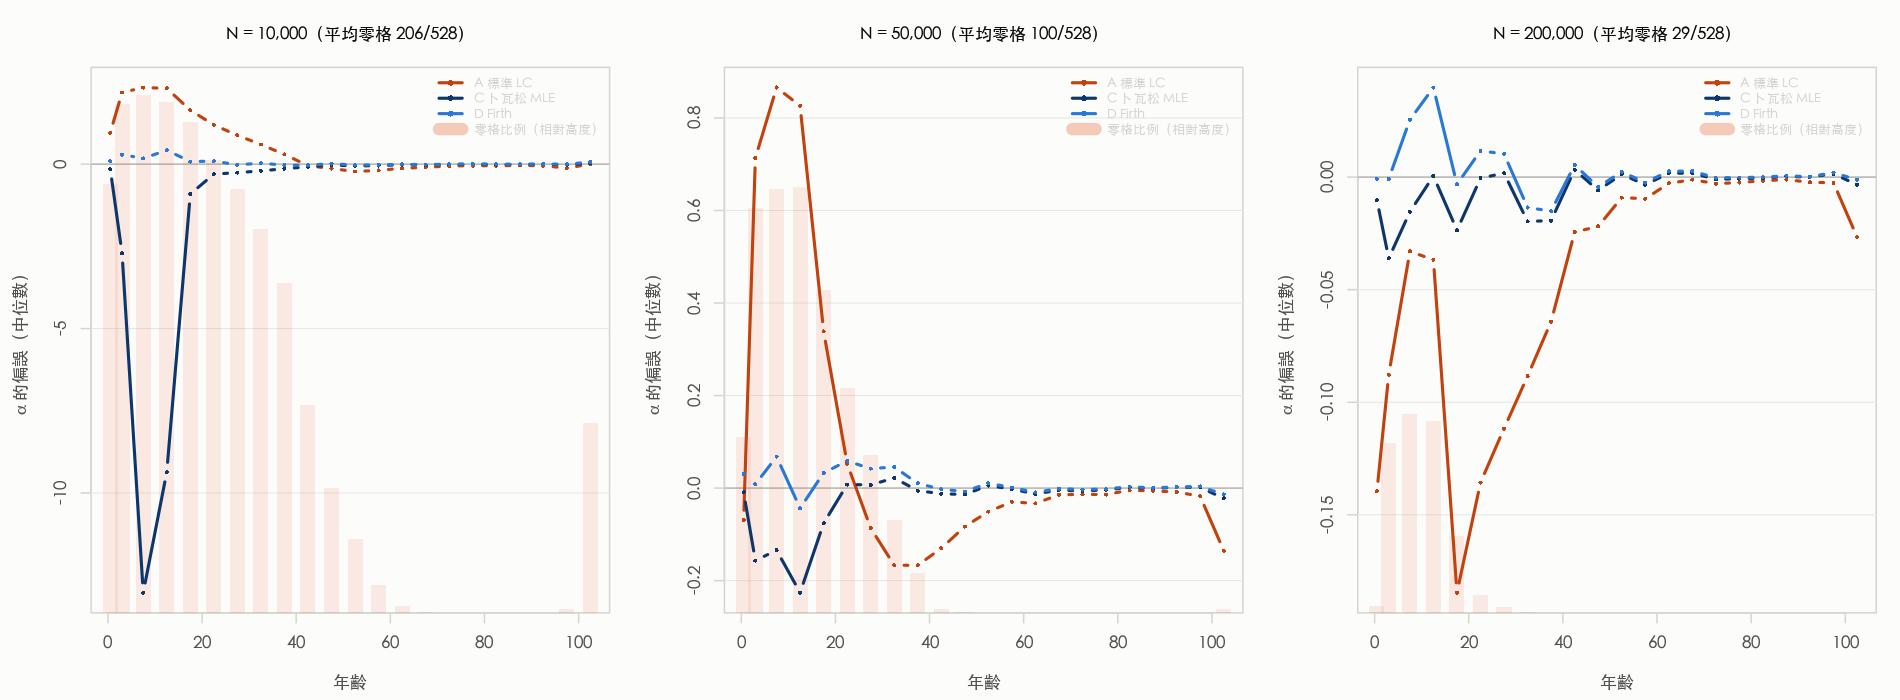
\includegraphics[width=\textwidth]{figH_eda_vs_alpha_bias.png}
  \caption{逐年齡的 $\alpha$ 偏誤（折線）與零死亡格比例（淺色柱，相對高度）。
  標準 LC 的偏誤峰值與零格所在的年齡完全重疊；卜瓦松在同處往反方向發散；
  Firth 則近乎水平。}
  \label{fig:edabias}
\end{figure}

零格比例與 $|\alpha$ 偏誤$|$ 的逐年齡 Spearman 相關，標準 LC 在三個規模下
分別為 0.863、0.881、0.740。\textbf{亦即\S\ref{sec:diag}圖中 T-ratio 的
尖峰位置，不需要真值、不需要一千次模擬，看診斷\cn{2}即可事前指出。}

此處有一項判讀上的陷阱須明說。Firth 的 Spearman 相關在 $N=10^4$ 時為
0.915，並不低於標準 LC。\textbf{但這不表示 Firth 沒有改善}——Spearman
相關對尺度不變，衡量的是「偏誤落在哪些年齡」而非「偏誤有多大」。Firth 改善的
是同一批年齡上的\textbf{量級}（最大偏誤 2.33 降至 0.43）。值得注意的是
Firth 的相關隨人口增大而下降（0.915、0.789、0.484），顯示其殘餘偏誤在大
人口下已不再由零格驅動。

\subsubsection{（五）加權只修漂移項，不修 $\alpha_x$}

變體 B 與 A 的對照是本節最乾淨的一項證據。$N=5\times10^4$ 時，把權重加入
高斯路線之後：

\begin{itemize}[leftmargin=*]
  \item 漂移項偏誤由 0.3339 降至 0.1223（2.7 倍），SSE($\beta$) 由
        4.449 降至 0.904（4.9 倍）；
  \item 但 $\alpha$ 的最大偏誤\textbf{紋風不動}——0.8658 對 0.8723。
\end{itemize}

因為加權完全沒有觸及零格與對數轉換。這與\S\ref{sec:decomp}變體 E
（不取對數但不加權，$\alpha$ 偏誤歸零而漂移項偏誤最大）恰成互補的一對，
合起來確立本文的核心分工：

\begin{quote}
\textbf{取對數傷 $\alpha_x$，不加權傷漂移項。} 前者須換分配假設或施以偏誤
減少，後者須引入資訊加權；兩者是獨立的病，也需要獨立的藥。
\end{quote}

\subsubsection{（六）$\beta_x$：門檻以上才有救，且必須靠收縮}

$N=10^4$ 時五種估計量的 cor($\beta$) 全在 0.125 以下，與診斷\cn{4}的
「不可還原」判讀一致——此規模下應誠實地不予估計。

$N=5\times10^4$ 起情況改變。標準 LC 的 0.037 確實與隨機方向無異，
但 Firth 加上 Fay-Herriot 收縮後可達 0.542，SSE 由 4.449 降至 0.143
（31 倍）。$N=2\times10^5$ 時則由 0.379 提升至 0.697。

收縮之所以有效，正因為\S\ref{sec:diag}已指出 $\beta_x$ 在此規模是
\textbf{變異數主導}；而 Fay-Herriot 的收縮強度由估計出的變異成分決定，
\textbf{沒有調校參數}，因而避開了本文議題三所指的選參準則錯置問題。

\subsubsection{（七）限制}

\begin{enumerate}[leftmargin=*]
  \item \textbf{真值的定義依賴估計量。} 本節以卜瓦松配適為真值
        （漂移 $-0.4087$），而\S\ref{sec:decomp}的階梯分解以 SVD 配適
        為真值（漂移 $-0.3678$）。兩表的漂移偏誤\textbf{不可跨表比較}，
        各自內部則一致。統一真值的定義為後續工作。
  \item \textbf{發散的處理。} 本節以 $|\hat\kappa|<10^3$ 為發散判準，
        三個規模下五種估計量皆無發散。惟 $N=10^4$ 時卜瓦松的 $-13.03$
        即是未被此判準剔除的近發散案例，該列應讀作「卜瓦松在此規模不可用」，
        而非其偏誤的可靠估計。
  \item \textbf{Fay-Herriot 的可交換先驗。} $\beta_x\sim N(1/A,A_\tau)$
        假設各年齡可交換，但真實的 $\beta_x$ 有明確的年齡結構。目前結果
        顯示此假設仍足以改善估計，更貼切的作法需引入相鄰年齡的相關性，
        等價於回到差分懲罰。
\end{enumerate}

\subsection{估計後的校正}\label{sec:postcorr}

老師另指出應探討\textbf{模型估計之後的校正}。本小節檢驗最直接的作法：
參數式拔靴法的偏誤校正
\begin{equation}
\tilde\theta=\hat\theta-\big(\bar\theta^{*}-\hat\theta\big)=2\hat\theta-\bar\theta^{*},
\end{equation}
其中 $\bar\theta^{*}$ 為自配適模型重抽所得估計值的平均。

\begin{table}[H]
\centering
\caption{參數式拔靴法偏誤校正的效果（重複 150 次，每次拔靴 60 次）}
\small
\begin{tabular}{lrrrr}
\toprule
 & \multicolumn{2}{c}{$N=5\times10^4$} & \multicolumn{2}{c}{$N=2\times10^5$}\\
\cmidrule(lr){2-3}\cmidrule(lr){4-5}
指標 & 未校正 & 校正後 & 未校正 & 校正後\\
\midrule
$\beta$ 的偏誤平方和 & 0.0708 & \textbf{0.0202} & 0.0092 & \textbf{0.0054}\\
$\beta$ 的 SSE 中位數 & \textbf{0.4628} & 0.5682 & 0.0583 & \textbf{0.0428}\\
漂移項偏誤 & 0.308 & 0.291 & 0.178 & 0.137\\
\bottomrule
\end{tabular}
\label{tab:postcorr}
\end{table}

\textbf{結果為混合。} 校正確實\textbf{降低了偏誤}——$\beta$ 的偏誤平方和
在兩個規模下分別下降 71\% 與 41\%，顯示參數式拔靴\textbf{確能偵測到
相當部分的偏誤}。但校正的代價是\textbf{放大變異數}：
$2\hat\theta-\bar\theta^{*}$ 此一線性組合的變異數約為原估計量的兩倍，
因此 $N=5\times10^4$ 時總誤差反而上升（SSE 中位數 0.463 $\to$ 0.568）；
須至 $N=2\times10^5$ 變異數較小時，淨效果才轉為正向
（0.0583 $\to$ 0.0428）。漂移項的偏誤則改善有限。

\textbf{此一結果修正了本文早期的論述。} 先前主張「拔靴法繞著已經偏掉的
配適值重抽，偵測不到自己的偏誤」，語氣過強；
正確的陳述應為：\textbf{參數式拔靴確能偵測到偏誤（偏誤平方和降七成），
但偏誤校正本身會放大變異數，故在變異數本已過大的小樣本下並不划算}。
此與\S\ref{sec:isrc} 所觀察到的「加入參數不確定性反而使涵蓋率下降」是同一件事的
兩種表現。

\noindent 實務建議因而是：\textbf{在 $N\ge2\times10^5$ 時可考慮拔靴偏誤校正，
更小的規模則應優先改用卜瓦松最大概似}（\S\ref{sec:decomp}），
自源頭避免偏誤，而非事後校正。

\section{懲罰式 Lee-Carter 模型}

本節回應\textbf{問題三}：將懲罰項直接加在年齡參數 $\boldsymbol{\beta}$ 上
是否可行，以及 LASSO、Ridge、Elastic Net 三者應如何取捨。

此一問題承接第陸節的結論。既然小樣本下的困難是偏誤而非變異數，
而懲罰式估計的本質正是\textbf{以偏誤換取變異數}，兩者看似方向相反；
但第陸節同時顯示 $\beta_x$ 的變異數在 $N\le20$ 萬時大到估計值完全不可用
（相關中位數低於 0.6），此時\textbf{即使引入額外偏誤，只要變異數的下降
足夠大，總均方誤差仍可能改善}。本節即在檢驗此一推論，並釐清三種懲罰在
「精確度」與「可解釋性」之間的權衡位置。

\subsection{模型設定}

在卜瓦松架構下加入 $\beta_x$ 的懲罰項：
\begin{equation}
\min_{\alpha,\beta,\kappa}\ -\ell(\alpha,\beta,\kappa)
+\lambda\sum_x w_x\Big[a\,|\beta_x-\beta_{0x}|
+\tfrac{1-a}{2}(\beta_x-\beta_{0x})^2\Big],
\quad \text{s.t. } \sum_x\beta_x=1,\ \sum_t\kappa_t=0,
\end{equation}
其中 $a=1$ 為 LASSO、$a=0$ 為 Ridge、$0<a<1$ 為 Elastic Net；
$w_x$ 為年齡別權重（可取 $1$ 或自適應權重 $1/\sqrt{D_{x\cdot}}$，
後者對應 Zou (2006) 的 adaptive LASSO）；$\beta_0$ 為收縮目標。

\subsection{收縮目標必須為非零向量}\label{sec:degenerate}

\textbf{此為實作上的關鍵前提。} 在 LC 的識別條件 $\sum_x\beta_x=1$ 之下，
若取 $\beta_0=\mathbf{0}$（即一般 LASSO 的預設），則
\begin{equation}
\sum_x|\beta_x|=\sum_x\beta_x+2\sum_x\max(-\beta_x,0)
=1+2\sum_x\max(-\beta_x,0).
\end{equation}
亦即 $L_1$ 懲罰項\textbf{只懲罰 $\beta_x$ 的負部，對正值完全沒有作用}。
當 $\hat\beta_x$ 全為正（人口規模較大時必然如此），$\sum_x|\beta_x|\equiv1$
為常數，懲罰項不影響 argmin，\textbf{估計值完全不動}。表~\ref{tab:shrink} 的數值驗證
顯示，$\lambda$ 由 $0$ 加到 $10^6$，估計值的變動量始終在機器精度
（$10^{-15}$）之內。Ridge 朝 $\mathbf{0}$ 收縮亦會退化為朝均勻向量收縮。

\begin{table}[H]
\centering
\caption{收縮目標的選擇（女性 2001$\sim$2024 年）}
\small
\begin{tabular}{rcccc}
\toprule
& \multicolumn{2}{c}{$\beta_0=\mathbf{0}$} & \multicolumn{2}{c}{$\beta_0=\mathbf{1}/A$}\\
\cmidrule(lr){2-3}\cmidrule(lr){4-5}
$\lambda$ & $\max|\hat\beta-\hat\beta^{\text{unpen}}|$ & 自由參數 &
            $\max|\hat\beta-\hat\beta^{\text{unpen}}|$ & 自由參數\\
\midrule
$0$      & --- & 22 & --- & 22\\
$10^2$   & $9.0\times10^{-17}$ & 22 & 0.0041 & 19\\
$10^4$   & $1.5\times10^{-16}$ & 22 & 0.0612 & 6\\
$10^6$   & $2.1\times10^{-15}$ & 22 & 0.0612 & 0\\
\bottomrule
\end{tabular}
\label{tab:shrink}
\end{table}

本文因此取 $\beta_0=\mathbf{1}/A$（均勻向量）。此一選擇有三項優點：
(1) $\sum_x\beta_{0x}=1=\sum_x\beta_x$，故 $\sum_x(\beta_x-\beta_{0x})=0$，
$\sum_x|\beta_x-\beta_{0x}|$ 並非常數，懲罰項有效；
(2) 具明確的人口學意義——$\beta_0=\mathbf{1}/A$ 代表
\textbf{「各年齡以相同速度改善」的虛無假設}，$\lambda\to\infty$ 時
$\hat\beta_x\to1/A$；
(3) LASSO 的稀疏性因而回答\textbf{「哪些年齡組的改善速度顯著偏離平均」}，
正是指導方向所期待的解釋效果。

若改取 $\beta_0=\hat\beta^{\text{ref}}$（參考母體的估計值），則本方法即成為
「依年齡決定是否併向參考母體」的變數選擇程序，可直接呼應
Yue et al.（2019）在結論中提出的建議。

\subsection{演算法與收斂性}

本文以區塊座標下降（Block Coordinate Descent）求解：$\alpha$ 有封閉解，
$\kappa$ 以 Newton 法更新後置中，$\beta$ 則以 proximal Newton
（二次近似加近端算子）更新——給定 Lagrange 乘子 $\nu$，各年齡的解為
\begin{equation}
\beta_x=\beta_{0x}+\frac{S\big(W_x(\tilde\beta_x-\beta_{0x})-\nu,\;
\lambda a w_x\big)}{W_x+\lambda(1-a)w_x},
\end{equation}
其中 $S(z,\gamma)=\mathrm{sign}(z)\max(|z|-\gamma,0)$ 為軟閾值算子，
$W_x=\sum_t\hat\mu_{xt}\kappa_t^2$ 為負二階導，$\nu$ 以二分法求解使
$\sum_x\beta_x=1$。每步並以步長折半確保目標函數不下降。

由於不可微的懲罰項僅作用於 $\beta$ 這一個區塊、且在各年齡間可分離
（separable），Tseng（2001）關於區塊座標下降的收斂定理適用，可保證每個
聚點皆為駐點。實測結果（表~\ref{tab:conv}、圖~\ref{fig:conv}）顯示：目標函數單調上升，
$\log_{10}\max_x|\Delta\beta_x|$ 隨迭代次數線性下降，即\textbf{幾何收斂}；
且\textbf{懲罰強度越大收斂越快}（$\lambda=0$ 需 33 次、$\lambda=10^3$ 需 18 次、
$\lambda=10^4$ 僅需 6 次），因為懲罰項改善了 Hessian 的條件數。

\begin{table}[H]
\centering
\caption{迭代收斂情形（女性 2001$\sim$2024 年，$\tau=10^{-11}$）}
\small
\begin{tabular}{rccc}
\toprule
$\lambda$ & 迭代次數 & 收斂 & 最終 $\max_x|\Delta\beta_x|$\\
\midrule
$0$      & 33 & 是 & $8.0\times10^{-6}$\\
$10^3$   & 18 & 是 & $1.2\times10^{-5}$\\
$10^4$   & \phantom{0}6 & 是 & $5.9\times10^{-7}$\\
\bottomrule
\end{tabular}
\label{tab:conv}
\end{table}

\begin{figure}[H]
\centering
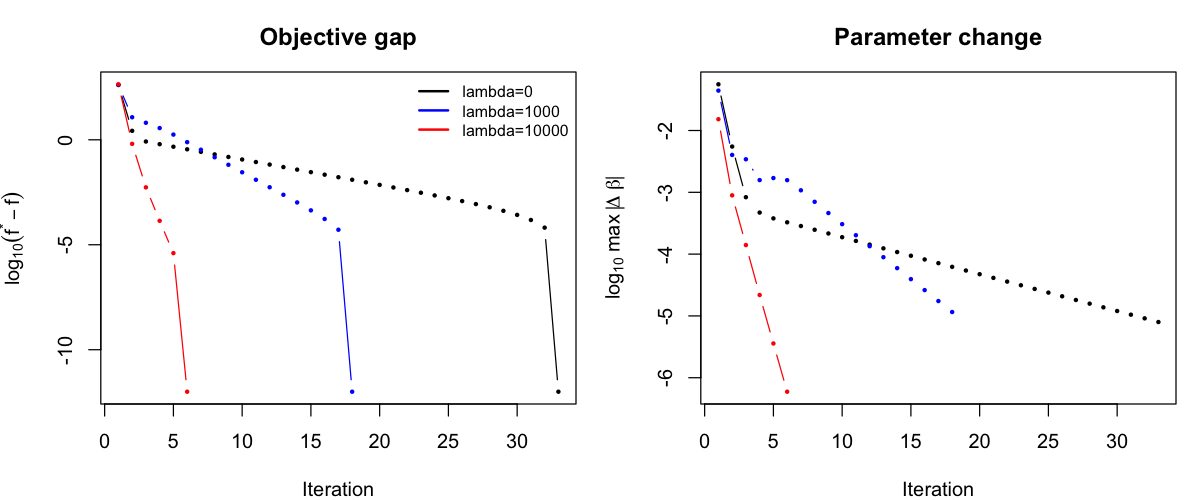
\includegraphics[width=0.88\textwidth]{fig1_convergence.png}
\caption{迭代收斂診斷。左：目標函數與最終值的間隙（對數尺度）；
右：參數變動量。兩者皆呈線性下降，即幾何收斂。}
\label{fig:conv}
\end{figure}

\subsection{係數路徑與稀疏性}

圖~\ref{fig:path} 左圖為 LASSO 的係數路徑：$\lambda$ 增大時各 $\hat\beta_x$ 依序被吸到
$1/A\approx0.0455$（虛線）。中圖顯示 Elastic Net 的稀疏化較 LASSO 緩慢，
此即 Zou and Hastie（2005）所述的群組效應（Grouping Effect）——相鄰年齡組的
$\beta_x$ 高度相關，純 LASSO 傾向任意只保留其中之一，而 $L_2$ 項使整組一同
保留。右圖的 BIC 在全國女性資料上偏好較小的 $\lambda$，此結果合理：
臺灣女性約 1,190 萬人，本即不需要收縮，\textbf{懲罰項的價值須在小人口才顯現}。

\begin{figure}[H]
\centering
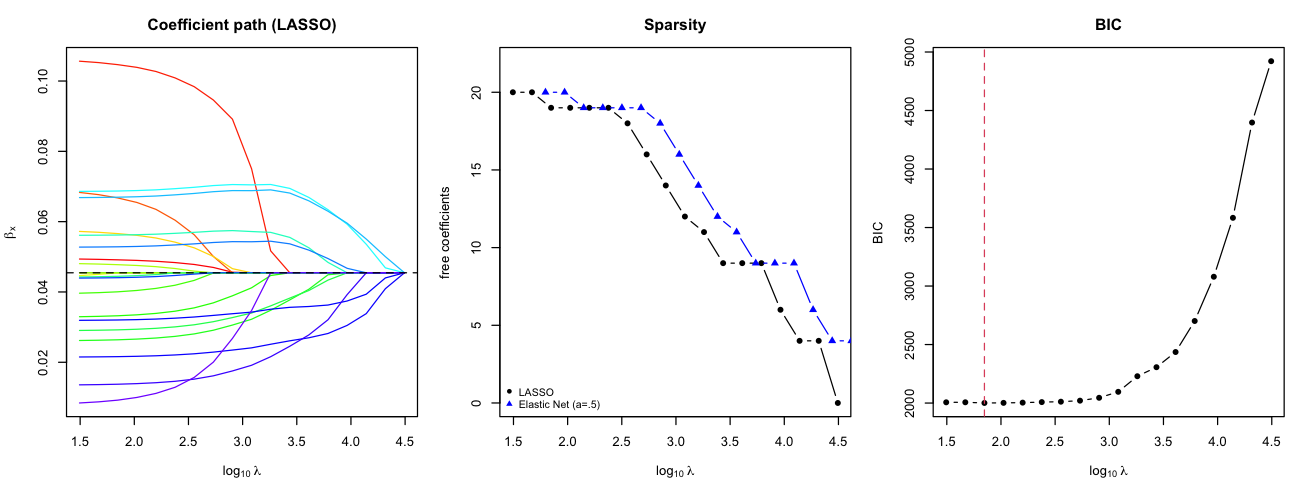
\includegraphics[width=\textwidth]{fig2_path.png}
\caption{LASSO 的係數路徑、稀疏度與 BIC（女性 2001$\sim$2024 年）}
\label{fig:path}
\end{figure}

\subsection{偏誤與變異數的權衡}

\textbf{懲罰強度須以 $\lambda_{\max}$ 正規化。} 概似函數的 Hessian 尺度正比於
暴露數 $N$，故絕對尺度的 $\lambda$ 在不同 $N$ 之間並不可比。本文依
Friedman et al.（2010）的作法，對每個模擬資料集各自計算使所有 $\beta_x$
皆被吸到 $\beta_0$ 的最小值 $\lambda_{\max}$，再以比例 $\lambda/\lambda_{\max}$
指定懲罰強度。

表~\ref{tab:bv} 與圖~\ref{fig:bv} 把 $\beta$ 的均方誤差拆成偏誤平方與
變異數兩項，用以檢驗前述推論。\textbf{三項指標的走向各自對應不同的判讀}：
變異數隨 $\lambda$ 下降代表收縮確實在穩定估計；偏誤平方隨 $\lambda$ 上升
代表收縮開始扭曲真實的年齡型態；\textbf{MSE 是兩者之和，其最小值的位置
即為最適的權衡點}。若 MSE 在 $\lambda=0$ 取最小，代表懲罰無益；
若在內部取最小，則代表\textbf{以偏誤換變異數確實划算}，即本節推論成立。

觀察結果，MSE 在兩個人口規模下\textbf{都在內部取得最小值}
（$N=5$ 萬時於 $\lambda/\lambda_{\max}=0.20$、$N=20$ 萬時於 0.03），
\textbf{與推論吻合}。

\begin{table}[H]
\centering
\caption{$\beta$ 的偏誤—變異數分解（LASSO，重複 100 次）}
\small
\begin{tabular}{rcccc}
\toprule
$N$ & $\lambda/\lambda_{\max}$ & 偏誤$^2$ & 變異數 & MSE\\
\midrule
50,000  & 0（未懲罰） & 0.00239 & 0.15980 & 0.16058\\
        & 0.10 & 0.00648 & 0.00512 & 0.01155\\
        & \textbf{0.20} & 0.00854 & 0.00158 & \textbf{0.01010}\\
        & 1.00 & 0.01066 & $2.8\times10^{-6}$ & 0.01066\\
\midrule
200,000 & 0（未懲罰） & 0.00024 & 0.01691 & 0.01698\\
        & 0.01 & 0.00015 & 0.01062 & 0.01066\\
        & \textbf{0.03} & 0.00147 & 0.00560 & \textbf{0.00702}\\
        & 0.10 & 0.00707 & 0.00102 & 0.00808\\
\bottomrule
\end{tabular}
\label{tab:bv}
\end{table}

\begin{figure}[H]
\centering
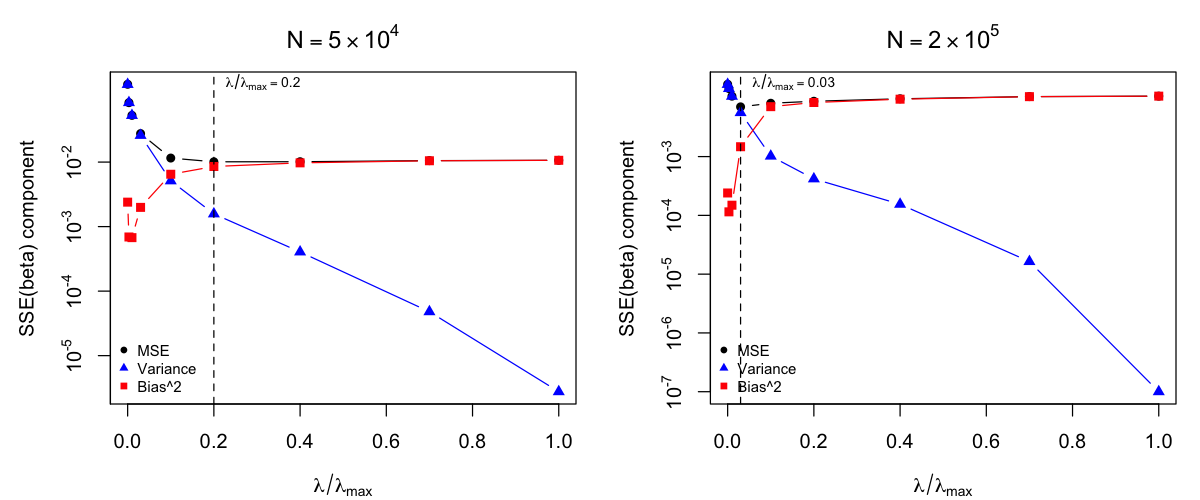
\includegraphics[width=0.92\textwidth]{fig3_bias_variance.png}
\caption{偏誤—變異數權衡（LASSO，重複 100 次）；虛線為 MSE 的最小值位置}
\label{fig:bv}
\end{figure}

兩項發現值得強調。其一，\textbf{在小人口時懲罰帶來的 MSE 改善極為可觀}：
$N=5$ 萬時最適 $\lambda/\lambda_{\max}=0.20$，MSE 由 0.1606 降至 0.0101
（\textbf{降低 94\%}），其中變異數降低 99\%，而偏誤平方僅由 0.0024 升至
0.0085。此即 James and Stein（1961）「以偏誤換變異數可使總 MSE 下降」的
古典結果在 LC 模型上的體現。其二，\textbf{最適懲罰強度隨 $N$ 增大而下降}
（$0.20\to0.03$），與理論一致。

\subsection{變異數的收斂速度}

固定 $\lambda/\lambda_{\max}=0.1$，比較未懲罰與懲罰版的變異數隨 $N$ 的變化
（表~\ref{tab:rate}、圖~\ref{fig:rate}）。以 $\log\mathrm{Var}$ 對 $\log N$ 迴歸，未懲罰版的斜率為
$-1.77$（標準誤 0.22），懲罰版為 $-1.27$（標準誤 0.04）。

\begin{table}[H]
\centering
\caption{變異數與 MSE 隨暴露數的變化（重複 100 次）}
\small
\begin{tabular}{rcccc}
\toprule
 & \multicolumn{2}{c}{未懲罰} & \multicolumn{2}{c}{LASSO ($\lambda/\lambda_{\max}=0.1$)}\\
\cmidrule(lr){2-3}\cmidrule(lr){4-5}
$N$ & 變異數 & MSE & 變異數 & MSE\\
\midrule
20,000    & 4.3912 & 4.3860 & \textbf{0.0223} & \textbf{0.0286}\\
50,000    & 0.2139 & 0.2148 & \textbf{0.0060} & \textbf{0.0119}\\
100,000   & 0.0526 & 0.0530 & \textbf{0.0021} & \textbf{0.0089}\\
200,000   & 0.0184 & 0.0184 & \textbf{0.0009} & \textbf{0.0081}\\
500,000   & 0.0066 & \textbf{0.0066} & 0.0003 & 0.0078\\
1,000,000 & 0.0030 & \textbf{0.0030} & 0.0001 & 0.0077\\
\midrule
\multicolumn{1}{l}{log-log 斜率} & $-1.77$ & & $-1.27$ & \\
\bottomrule
\end{tabular}
\label{tab:rate}
\end{table}

\begin{figure}[H]
\centering
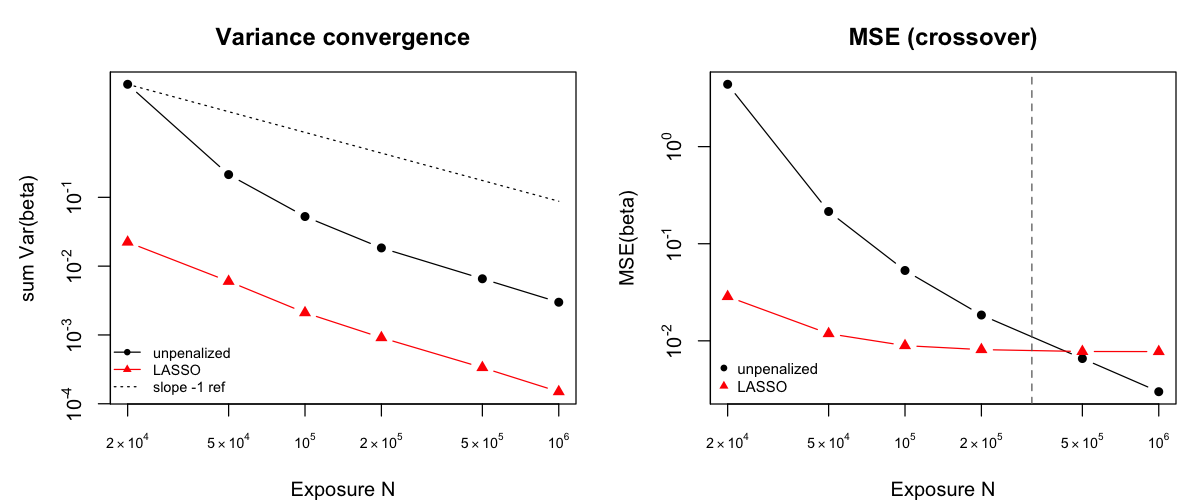
\includegraphics[width=0.92\textwidth]{fig4_variance_rate.png}
\caption{變異數的收斂速度與 MSE 的交叉（重複 100 次）}
\label{fig:rate}
\end{figure}

三項發現如下。

\textbf{其一，懲罰項大幅降低變異數的「常數項」，而非改變其收斂階數。}
$N=2$ 萬時未懲罰版的變異數為 4.391，懲罰版僅 0.022，相差約 \textbf{197 倍}；
但兩者的 log-log 斜率均在 $-1.3$ 至 $-1.8$ 之間，並未出現階數上的差異。
值得注意的是未懲罰版的斜率標準誤（0.22）遠大於懲罰版（0.04），
顯示未懲罰版在小 $N$ 並非穩定的冪次關係，而是處於\textbf{崩潰區}——
其「較陡的斜率」實為脫離崩潰區的過渡，不宜解讀為收斂較快。

\textbf{其二，固定比例的懲罰在大人口會反過來損害 MSE。} 由於偏誤不隨 $N$
消失（固定 $\lambda/\lambda_{\max}$ 使懲罰強度與概似同步成長），懲罰版的 MSE
在 $N\ge5\times10^5$ 後停滯於 0.0077 左右，而未懲罰版持續下降至 0.0030。
兩者的\textbf{交叉點約在 $N=3\times10^5$}。

\textbf{其三，因此 $\lambda$ 必須隨 $N$ 調整。} 表~\ref{tab:bv} 已顯示最適比例由
$N=5$ 萬時的 0.20 降至 $N=20$ 萬時的 0.03。實務上建議以第陸節之二所述的
參數式拔靴插入式選法選取，而非固定比例。

\subsection{三種懲罰的比較}

表~\ref{tab:pen} 為 $N=20$ 萬、各懲罰以自身的 $\lambda$ 格點搜尋至 MSE 最小的結果。

\begin{table}[H]
\centering
\caption{三種懲罰的比較（$N=20$ 萬，重複 100 次，各取其最適 $\lambda$）}
\small
\begin{tabular}{lcccccc}
\toprule
懲罰 & $a$ & 最適 $\lambda/\lambda_{\max}$ & 偏誤$^2$ & 變異數 & MSE & $\beta$ 相關中位數\\
\midrule
未懲罰 & --- & 0 & 0.00024 & 0.01691 & 0.01698 & 0.711\\
LASSO & 1.0 & 0.030 & 0.00147 & 0.00560 & 0.00702 & 0.703\\
Elastic Net & 0.5 & 0.030 & 0.00158 & 0.00534 & 0.00687 & 0.705\\
Ridge & 0.0 & 0.003 & 0.00270 & 0.00311 & \textbf{0.00578} & \textbf{0.721}\\
\bottomrule
\end{tabular}
\label{tab:pen}
\end{table}

三者相對於未懲罰版的 MSE 分別降低 59\%、60\% 與 66\%。
\textbf{值得注意的是，若目標純粹為降低 $\beta$ 的 MSE，Ridge 的表現最佳}，
LASSO 反而最差。其原因在於真值 $\beta_x$ 並無任何一組恰等於 $1/A$——
亦即\textbf{稀疏性並非正確的先驗}，而 Ridge 的純收縮更貼近實情。

然而這並不代表 LASSO 沒有價值。LASSO 提供 Ridge 所沒有的\textbf{變數選擇與
可解釋性}：它能明確指出哪些年齡組的改善速度顯著偏離平均（表~\ref{tab:shrink} 顯示
$\lambda=10^4$ 時僅 6 個年齡組維持自由）。在均方誤差與可解釋性之間的
權衡約為 20\%，是否值得取決於研究目的。若目的為\textbf{估計精確度}，宜採
Ridge 或 Elastic Net；若目的為\textbf{辨識關鍵年齡組}，則 LASSO 為適當選擇。
Elastic Net 兼具兩者，且其 MSE 與 Ridge 接近，或為折衷方案。

\subsection{Elastic Net 的其他變體}

由於前一小節顯示 LASSO 的弱點在偏誤，本文另外試驗三種以「降低收縮偏誤」
為目的的變體，並與 LASSO、Elastic Net 並列（表~\ref{tab:variants}）：

\begin{itemize}
  \item \textbf{自適應 LASSO}（Zou 2006）：以未懲罰估計的偏離量倒數為權重，
        $w_x=1/|\hat\beta_x^{\text{unpen}}-\beta_{0x}|$，使證據較強的年齡組
        受到較輕的懲罰。
  \item \textbf{鬆弛 LASSO}（Meinshausen 2007）：先以 LASSO 選出作用集，
        再於作用集上不加懲罰重新配適，非作用集固定於 $\beta_0$。
  \item \textbf{MCP}（Zhang 2010）：非凸懲罰，其導數隨 $|\beta_x-\beta_{0x}|$
        增大而遞減至零，因而保留稀疏性卻不對大係數施加偏誤。
\end{itemize}

\begin{table}[H]
\centering
\caption{Elastic Net 族各變體的比較（$N=20$ 萬，重複 100 次，各取其最適 $\lambda$）}
\small
\begin{tabular}{lcccc}
\toprule
方法 & 最適 $\lambda/\lambda_{\max}$ & 偏誤$^2$ & 變異數 & MSE\\
\midrule
Ridge（前表） & 0.003 & 0.00270 & 0.00311 & \textbf{0.00578}\\
LASSO & 0.03 & 0.00219 & 0.00484 & 0.00698\\
MCP（$\gamma=3$） & 0.03 & 0.00219 & 0.00485 & 0.00698\\
Elastic Net & 0.10 & 0.00463 & 0.00255 & 0.00716\\
自適應 LASSO & 0.40 & 0.00313 & 0.00532 & 0.00840\\
鬆弛 LASSO & 0.20 & 0.00734 & \textbf{0.00192} & 0.00924\\
\bottomrule
\end{tabular}
\label{tab:variants}
\end{table}

三項觀察。其一，\textbf{沒有任何一個稀疏型變體能勝過單純的 Ridge}。
這與前一小節的診斷一致：真值 $\beta_x$ 並無恰等於 $1/A$ 者，
問題本質是\textbf{稠密}的，因此所有為稀疏性設計的機制都無從發揮。
其二，\textbf{MCP 與 LASSO 幾乎完全相同}（MSE 差異在第四位小數）。
原因是在最適的 $\lambda$ 之下閾值本就很小，MCP「對大係數不加偏誤」的區段
極少被觸發，退化為 LASSO。其三，\textbf{鬆弛 LASSO 的變異數最低卻 MSE 最差}
——它把非作用集\textbf{硬性固定}於 $\beta_0$，等於施加一個過強的等式限制，
偏誤平方因而升至 0.0073。

\subsection{點估計 LASSO 與分位數 LASSO 的演算法差異}\label{sec:algodiff}

本文在兩處用到 $L_1$ 懲罰，但兩者的最佳化結構\textbf{並不相同}，
可用的演算法也不相同。此一區分在文獻中常被「LASSO」一詞掩蓋，
卻直接決定了實作的可行性，故於此釐清。

\subsubsection{（一）兩種問題的結構}

\textbf{點估計 LASSO}（本文第柒節所用）以平滑的損失搭配 $L_1$ 懲罰：
\begin{equation}\label{eq:pointlasso}
\min_{\boldsymbol{\beta}}\ \underbrace{-\ell(\boldsymbol{\beta})}_{\text{可微}}
+\underbrace{\lambda\textstyle\sum_x w_x|\beta_x-\beta_{0x}|}_{\text{不可微，但逐座標可分離}} .
\end{equation}

\textbf{分位數 LASSO}（\S\ref{sec:rmmethod} 所述的修勻）則以檢查函數
$\rho_\tau(u)=u(\tau-\mathbf{1}\{u<0\})$ 為損失：
\begin{equation}\label{eq:qlasso}
\min_{z}\ \underbrace{\textstyle\sum_i\rho_\tau(y_i-(Mz)_i)}_{\text{不可微，且耦合所有座標}}
+\lambda\|Dz\|_{L_1}.
\end{equation}

兩者的關鍵差別在於\textbf{不可微的部分落在哪裡}。
式~\eqref{eq:pointlasso} 的不可微項是懲罰，逐座標分離；
式~\eqref{eq:qlasso} 的不可微項是\textbf{損失本身}，而
$\rho_\tau(y_i-(Mz)_i)$ 把所有座標耦合在內積 $(Mz)_i$ 之中，無法分離。

\subsubsection{（二）Tseng（2001）的條件與其違反}

Tseng（2001）的收斂定理要求目標函式可寫成
\begin{equation}\label{eq:tseng}
f(x_1,\dots,x_N)=f_0(x_1,\dots,x_N)+\sum_{k=1}^{N} f_k(x_k),
\end{equation}
其中 $f_0$ 可微、不可微的 $f_k$ 逐區塊可分離。該文並明白指出：

\begin{quote}\small
「若 $f$ 不可微，座標下降法\textbf{可能卡在非駐點，即使 $f$ 為凸}……
因此一般認為該方法不適用於不可微的情形。
\textbf{惟當 $f$ 的不可微部分可分離時則為例外。}」
（Tseng 2001: 475，本文中譯）
\end{quote}

對照可知：式~\eqref{eq:pointlasso} 符合式~\eqref{eq:tseng} 的形式，
故第柒節之三的區塊座標下降有收斂保證；
式~\eqref{eq:qlasso} 則\textbf{不符合}，座標下降並無保證。

\subsubsection{（三）以實際資料驗證卡滯}

上述為理論陳述，本文另以實際資料檢驗其是否真的發生。取女性
2015$\sim$2024 年（$22\times10=220$ 格）建構修勻問題，
對\textbf{同一個}目標函式式~\eqref{eq:qlasso} 施以兩種演算法，
結果如表~\ref{tab:algo}。

為避免「卡滯只是步長設定不良」的疑慮，此處的座標下降採用
\textbf{精確的單座標最小化}——$L_1$ 損失沿單一座標的最小值為加權中位數，
有封閉解，不涉及任何步長選擇。

\begin{table}[H]
\centering
\caption{同一目標函式下兩種演算法的比較（女性 2015$\sim$2024 年）}
\small
\begin{tabular}{llrcl}
\toprule
目標函式 & 演算法 & 目標值 & 是否達最適 & 診斷\\
\midrule
分位數 LASSO & 線性規劃（內點法） & \textbf{30.02} & 是 & ---\\
分位數 LASSO & 座標下降（精確） & \textbf{1244.20} & \textbf{否} & 可改善的單座標移動 $0/220$\\
\midrule
點估計 LASSO & 座標下降（軟閾值） & --- & 是 & KKT 最大違反 $7.1\times10^{-16}$\\
\bottomrule
\end{tabular}
\label{tab:algo}
\end{table}

座標下降在\textbf{第一次掃描後即停止，且目標值等於起始值}——換言之
完全沒有移動，而該點的目標值是線性規劃解的 \textbf{41.4 倍}。

\textbf{卡滯的機制可以明確指認。} 在起始點 $z=\mathbf{0}$ 處，
沿第 $j$ 個座標移動時，保真列貢獻權重 $1$、懲罰列貢獻權重
$\sum|D_{\cdot j}|$；本設定下後者的中位數為 $21.60$、最小值 $5.40$，
\textbf{全部 220 個座標的懲罰權重都大於保真權重}。
由於 $L_1$ 的單座標最小值為加權中位數，權重集中於「不動」的一側時
最小值即為 $0$，故\textbf{每個座標都同意不要移動}。
然而聯合移動可使目標值由 1244.20 降至 30.02——
此即典型的「對角山谷」：沿任一軸皆上坡，沿對角線則下坡。
本文逐一檢驗 220 個座標的八種位移，確認\textbf{無任何單座標移動可改善}，
證實此為結構性的卡滯而非實作缺陷。

對照之下，同一組資料改用平方損失搭配 $L_1$ 懲罰，座標下降
\textbf{兩次掃描即收斂}，KKT 條件的最大違反為 $7.1\times10^{-16}$，
確實達到最適。\textbf{兩者的差別純粹來自損失函數是否可微。}

\subsubsection{（四）對本文實作的意涵}

上述分析解釋了本文兩個模組為何採用不同的演算法，且此一選擇是
\textbf{結構決定的，而非實作偏好}：

\begin{table}[H]
\centering
\caption{本文兩個模組的目標函式與演算法}
\small
\begin{tabular}{lll}
\toprule
模組 & 目標函式 & 演算法\\
\midrule
\texttt{smooth\_l1\_2d()} & $L_1$ 損失 ＋ $L_1$ 懲罰 &
  \texttt{rq.fit.sfn}（Frisch--Newton 內點法）\\
\texttt{lc\_penalized()} & 卜瓦松對數概似 ＋ $L_1$ 懲罰 &
  proximal Newton ＋ 軟閾值\\
\bottomrule
\end{tabular}
\label{tab:modules}
\end{table}

三項延伸意涵值得記錄。

\textbf{其一，第柒節之三的收斂論證因此有了對照組。} 該處主張
「不可微的懲罰項僅作用於 $\boldsymbol{\beta}$ 這一個區塊、且在各年齡間
可分離，故 Tseng（2001）的定理適用」；表~\ref{tab:algo} 顯示，
若把損失換成 $L_1$，同一套演算法便會失效。此一對照使該主張
不再只是引用定理，而有了具體的反面證據。

\textbf{其二，$L_1$ 損失的選擇有其統計理由，非僅為計算方便。}
$\tau=0.5$ 的檢查函數等價於 Laplace 分配的最大概似，對離群值較平方損失
穩健；Schuette（1978）即以此為由主張以線性規劃處理修勻問題，
Dokumentov et al.（2018）沿用之，Rabbi and Mazzuco（2021）亦引述此點。
換言之，穩健性與「必須使用線性規劃」是同一個選擇的兩面。

\textbf{其三，解的性質不同。} 線性規劃的解落在可行域的頂點上，
意味著恰有若干筆殘差為零（曲面「內插」這些觀測值）；
平方損失的解則一般不內插任何一點。此一差異在解釋修勻後曲面的行為時
須留意，亦是 $L_1$ 修勻「較不平滑但誤差較小」（表~\ref{tab:smooth}）的
成因之一。

\subsection{小結：懲罰項該怎麼用}

綜合本節，對小人口 LC 模型施加懲罰的建議如下：

\begin{enumerate}[leftmargin=*]
  \item \textbf{收縮目標必須非零}，否則在 $\sum_x\beta_x=1$ 之下懲罰項退化。
  \item \textbf{若目標是估計精確度}，Ridge 或 Elastic Net 優於 LASSO；
        稀疏性在此問題上並非正確的先驗。
  \item \textbf{若目標是辨識關鍵年齡組}，LASSO 仍是唯一選擇，
        與均方誤差之間的權衡約為 20\%。
  \item \textbf{$\lambda$ 必須隨人口規模調整}，固定比例在大人口反而有害。
  \item \textbf{懲罰在 $N\le20$ 萬時效益最大}，此區間正是我國多數鄉鎮市區的
        規模，亦即本方法的實務適用範圍。
  \item \textbf{損失函數是否可微，決定了可用的演算法}（\S\ref{sec:algodiff}）：
        平滑損失搭配可分離懲罰可用座標下降，$L_1$ 損失則必須走線性規劃。
        此一區分在文獻中常被「LASSO」一詞掩蓋。
\end{enumerate}

\section{區間推論}\label{sec:interval}

本節回應\textbf{問題四}：小人口的預測區間誤差來自何處，以及文獻長期主張的「LC 區間過窄」在此是否成立。

須先說明本節與前兩節的關係。點估計的準確與區間的有效是兩個不同的性質，而且可能衝突——本文第伍節即顯示修勻改善了點估計卻破壞了區間，且代價隨人口增大而惡化。因此區間須獨立檢驗，不能由點估計的表現推得。

\subsection{來源分解：四個層層疊加的變體}\label{sec:isrc}

本小節針對議題二進行檢驗，並回應\S\ref{sec:est}留下的第二個環節：
點估計的偏誤如何傳導至預測區間。設定預測期 $h=10$、名目水準 80\%，目標為涵蓋真模型在觀測的
$\kappa_t$ 路徑下的 $e_0$。

\textbf{實驗設計}：區間的寬度與位置由多個誤差來源共同決定，單一組數字無法
辨識各成分的貢獻，本文因此設計\textbf{四個層層疊加的變體}，每次只加入一個
誤差來源：

\begin{itemize}
  \item \textbf{變體 O（不可約下限）}：假設參數全部已知，區間只反映
        $\kappa_t$ 未來的創新項。此為任何方法都無法低於的理論下限，
        \textbf{其涵蓋率應接近名目的 0.80}，可作為整個實驗的效度檢查。
  \item \textbf{變體 P（插入式）}：以估計出的 $\hat{\boldsymbol{\kappa}}$
        與 $\hat\sigma$ 代入，即現行實務作法。\textbf{P 與 O 的差距，
        即為「以估計值取代真值」所須付出的權衡}。
  \item \textbf{變體 B（加計參數不確定性）}：在 P 之上以拔靴法納入參數估計
        的不確定性。\textbf{若參數不確定性是區間失效的主因，B 應明顯優於 P}。
  \item \textbf{變體 S（加計修勻）}：在 B 之上先行修勻，
        \textbf{專門檢驗 Basellini et al.（2023）「修勻壓低歷史變異、
        使區間過窄」的疑慮}。
\end{itemize}

閱讀時須同時看兩個指標：\textbf{平均寬度}反映區間的大小、
\textbf{涵蓋率}反映區間是否擺對位置。兩者\textbf{必須合看}——寬度過大而
涵蓋率仍低，即代表位置錯誤而非寬度不足。結果如表~\ref{tab:decomp}。

\begin{table}[H]
\centering
\caption{預測區間寬度與涵蓋率的來源分解（名目 80\%）}
\small
\begin{tabular}{rlcc}
\toprule
$N$ & 變體 & 平均寬度 & 涵蓋率\\
\midrule
50,000 & O\quad 僅未來創新項（不可約下限） & 1.743 & 0.85\\
       & P\quad 插入式（現行作法） & 5.401 & 0.38\\
       & B\quad P ＋參數不確定性 & 6.166 & 0.24\\
       & S\quad 修勻 ＋ B & 1.683 & 0.66\\
\midrule
200,000 & O & 1.720 & 0.82\\
        & P & 5.651 & 0.82\\
        & S & 1.515 & 0.63\\
\midrule
1,000,000 & O & 1.738 & 0.77\\
          & P & 4.390 & 0.94\\
          & S & 1.194 & 0.45\\
\midrule
11,900,000 & O & 1.723 & 0.87\\
           & P & 1.950 & 0.88\\
           & S & \textbf{0.529} & \textbf{0.38}\\
\bottomrule
\end{tabular}
\label{tab:decomp}
\end{table}

\textbf{其一，小人口的預測區間同時「太寬」且「涵蓋不足」，寬度與涵蓋率解耦。}
$N=5$ 萬時現行作法的區間寬達 5.401（不可約下限僅 1.743），涵蓋率卻只有
0.38。寬度被灌水是因 $\hat\kappa_t$ 含估計雜訊、使一階差變大、$\hat\sigma$
被高估；涵蓋失敗則因漂移項被壓平，使區間\textbf{擺錯位置}。
換言之，\textbf{小人口的問題是偏誤而非寬度，加寬區間無濟於事}。此一結果
推翻了文獻長期以來「LC 模型預測區間過窄」的診斷在小人口的適用性。

\textbf{其二，拔靴法的參數不確定性幾乎沒有貢獻，有時甚至更糟}（變體 B）。
因為拔靴法是繞著已經偏掉的配適值重抽，\textbf{偵測不到自己的偏誤}。此一
現象在本文的模擬中出現三次，可作為貫穿全文的主題。

\textbf{其三，修勻確實使區間系統性過窄，且 $N$ 越大越嚴重}（涵蓋率由 0.66
降至 0.45 再降至 0.38；在實際資料規模時區間寬度 0.529 對不可約下限 1.723，
窄了逾三倍）。其機制是：小 $N$ 時修勻移除的是估計雜訊，大 $N$ 時已無雜訊
可移，移除的便是 $\kappa_t$ 真實的年際變動。
\textbf{此即 Basellini et al.（2023）提出但未量化的疑慮，本文提供了量化證據，
並指出其效應隨暴露數增大而惡化，方向與直覺相反。}

\subsection{兩步校正}\label{sec:twostep}

\subsubsection{（一）步驟一（位置）：以卜瓦松最大概似取代 SVD}

\begin{table}[H]
\centering
\caption{SVD 與卜瓦松最大概似的漂移項估計（真值 $-0.3678$）}
\small
\begin{tabular}{rcc}
\toprule
$N$ & SVD 的漂移項 & 卜瓦松 MLE 的漂移項\\
\midrule
50,000    & $-0.032$（偏誤 $+0.336$） & $\mathbf{-0.377}$（偏誤 $-0.010$）\\
200,000   & $-0.194$（偏誤 $+0.174$） & $\mathbf{-0.369}$（偏誤 $-0.002$）\\
1,000,000 & $-0.365$ & $-0.367$\\
\bottomrule
\end{tabular}
\label{tab:drift}
\end{table}

由表~\ref{tab:drift} 可知，\textbf{漂移項衰減並非小人口的固有性質，而是 SVD 對
$\log(D/E)$ 做最小平方所產生的結果}。卜瓦松架構不取對數，衰減即告消失。
此一發現獨立支持了 Basellini et al.（2023）「換到卜瓦松架構後第二階段調整
不再必要」的論點，並把理由由「配適總死亡數依照模型假設成立」推進到
\textbf{「避免小樣本的對數偏誤」}。

\subsubsection{（二）步驟二（寬度）：以拔靴法去除 $\hat\sigma$ 的估計雜訊}

由 $\hat\kappa_t=\kappa_t+u_t$ 可得
$\widehat{\mathrm{Var}}(\Delta\hat\kappa)\approx\sigma^2
+\mathrm{Var}(\Delta u)$，以參數式拔靴法估計 $\mathrm{Var}(\Delta u^*)$ 後
扣除即可。以真值 $\sigma=0.7496$ 為例，$N=20$ 萬時由 1.152 校正為
\textbf{0.702}，$N=100$ 萬時由 0.870 校正為 \textbf{0.751}。惟 $N=5$ 萬時
$\sqrt{V_u}=7.36$ 大於未校正的 $\hat\sigma=2.30$，兩個大噪音量相減並不穩定，
是動差法去偏的典型病症，因此\textbf{去偏約需 $N\ge20$ 萬方為可行}。

\subsubsection{（三）兩步合併後的校準結果}

\begin{table}[H]
\centering
\caption{校正前後的預測區間寬度與涵蓋率（名目 80\%）}
\small
\begin{tabular}{rlcc}
\toprule
$N$ & 方法 & 區間寬度 & 涵蓋率\\
\midrule
200,000 & oracle & 1.743 & 0.81\\
        & 現行作法 & 5.081 & 0.75\\
        & 本文校正版 & \textbf{1.724} & 0.63\\
\midrule
1,000,000 & oracle & 1.726 & 0.85\\
          & 現行作法 & 4.667 & 0.95\\
          & 本文校正版 & \textbf{1.721} & \textbf{0.83}\\
\midrule
11,900,000 & oracle & 1.712 & 0.78\\
           & 現行作法 & 2.033 & 0.82\\
           & 本文校正版 & \textbf{1.678} & 0.77\\
\bottomrule
\end{tabular}
\label{tab:calib}
\end{table}

$N\ge100$ 萬時，校正版的區間寬度幾乎完全追平不可約下限，涵蓋率 0.83 對名目
的 0.80 亦屬良好。相對地，現行作法在同一點雖有 0.95 的涵蓋率，卻是以 2.7
倍的寬度換來，並非校準良好。

惟 $N=20$ 萬時寬度雖已校正，涵蓋率仍僅 0.63。殘餘的位置誤差來自
$\hat\kappa_T$ 這個預測初始值本身——它是單一年份的估計值，誤差不隨配適期長度
$T$ 縮小。Lee and Miller（2001）的初始值修正正是在處理此事，而
Stoeldraijer et al.（2018）以八個歐洲國家的資料發現，初始值的選擇存在
準確度與穩健度的取捨。該取捨在小人口應如何拿捏，文獻中尚無量化研究，是本文
後續可補之處。


\section{結論與後續工作}

\subsection{結論}

本文以 Rabbi and Mazzuco（2021）為起點，在臺灣五齡組死亡資料上完成還原並
向外延伸，主要結論如下。

第一，該方法的優點部分成立：LASSO 修勻的配適精確度確實優於樣條，壽命差異
調整亦使 $\kappa_t$ 更接近線性。但這些優勢\textbf{僅在近期短配適期存在}，
配適期拉長後即被 Lee-Miller 方法超越，而原文並未檢驗配適期的敏感度。

第二，該方法的預測區間\textbf{不但未變窄，反而是六種方法中最寬者}，因為
「$\kappa_t$ 更線性」與「$\kappa_t$ 變異更小」並不等價，原文將兩者綁在一起
論述並不妥當。

第三，小人口下 LC 模型的失效\textbf{並非單一機制}。依第肆節的診斷與分解：
$\alpha_x$ 的偏誤確實來自 SVD 對小樣本取對數（移除對數後偏誤歸零）；
但\textbf{漂移項的偏誤與對數無關}——在完全不涉及對數的高斯對照下，
漂移項偏誤仍達 0.347，甚至略大於標準 LC 的 0.305，
其來源為主奇異向量對噪音的敏感性。至於 $\beta_x$，T-ratio 顯示其在小樣本
為\textbf{變異數}問題，待 $N\ge5\times10^5$ 變異數收斂後才轉為偏誤問題。
惟就預測區間而言結論不變：涵蓋失敗來自漂移項衰減造成的位置偏誤，
文獻共識「LC 模型的預測區間過窄」在小人口並不成立。此一發現呼應並補充了
Wang et al.（2018）與余清祥等（2021）關於 $\alpha_x$、$\beta_x$ 偏誤的研究，
並將討論延伸至 Yue et al.（2019）明白指出尚未處理的時間參數 $\kappa_t$。

第四，本文提出的兩步校正（卜瓦松最大概似取代 SVD、拔靴法去除 $\hat\sigma$
的估計雜訊）在 $N\ge100$ 萬時可使區間寬度幾乎追平理論下限，惟去偏步驟約
需 $N\ge20$ 萬方為可行。

第五，修勻確實會壓低預測區間寬度，且效應隨暴露數增大而惡化。此即
Basellini et al.（2023）提出但未量化的疑慮，本文提供了量化證據。

第六，關於懲罰式估計，本文有三項發現。其一，\textbf{在 LC 的識別條件
$\sum_x\beta_x=1$ 之下，朝零收縮的懲罰項退化為常數、完全不影響估計值}，
收縮目標必須取非零向量；本文取均勻向量 $\mathbf{1}/A$，其人口學意義為
「各年齡以相同速度改善」的虛無假設。其二，\textbf{懲罰項在小人口帶來的
改善極為可觀}——$N=5$ 萬時 $\beta_x$ 的均方誤差降低 94\%、變異數降低 99\%；
但懲罰主要縮小的是變異數的\textbf{常數項}而非其收斂階數，且固定比例的懲罰
在 $N\ge3\times10^5$ 後因偏誤不隨樣本數消失而反受其害，故 $\lambda$ 必須隨
人口規模調整。其三，\textbf{若目標純為降低均方誤差，Ridge 優於 LASSO}
（MSE 分別降低 66\% 與 59\%），因為真值 $\beta_x$ 並無恰等於 $1/A$ 者、
稀疏性並非正確的先驗；LASSO 的價值在於可解釋性，以約 20\% 的均方誤差
換取「哪些年齡組顯著偏離平均改善速度」的明確答案。

\subsection{研究限制}

\begin{enumerate}[leftmargin=*]
  \item \textbf{五齡組本身即是強力的變異數縮減器}（本文資料最小格死亡數 37、
        中位數 1,201）。因此所得門檻是「五齡組之下」的門檻，不宜與單齡組
        研究直接比較。惟我國鄉鎮市區資料多為五齡組，故此設定仍具實務意義。
  \item \textbf{配適期長度與人口規模已納入二因子設計}（\S\ref{sec:TN}），
        並發現前者更為關鍵。惟本文僅以最近 $T$ 年為窗口，未考慮窗口起點
        位置的影響（例如同樣 20 年，1970$\sim$1989 與 2005$\sim$2024 的
        死亡轉型速度不同）。
  \item \textbf{模擬的真值取自 LC 配適，隱含「模型正確」的假設}。真實小區域
        的 $\beta_x$ 可能本就異於全國，此部分異質性本設計無法衡量，因此模擬
        所得應視為下界。
  \item \textbf{涵蓋率的實證驗證本身有其困難}：資料在年齡與時間上均存在相關，
        單一人口留出期的涵蓋率屬高度相關的少數觀測。
  \item \textbf{留出期涵蓋 COVID-19}（女性 $e_0$ 於 2020 年達 84.30 歲，
        2022 年降至 83.14 歲，2024 年才回到 83.94 歲），屬真實的結構性衝擊。
  \item \textbf{模擬規模已統一}：本版所有蒙地卡羅一律重複 100 次、
        固定亂數種子（20260921），取代先前 8 至 50 次的試跑結果。
        第陸節的數值因此與早期版本略有出入，其中 $\lambda$ 選法的相對損失
        由「約七倍」修正為 3.49 倍，三方向格點的建議組合由 $(1,2,1)$
        改為 $(1,5,5)$；結論方向不變。
\end{enumerate}

\subsection{後續工作}

\begin{enumerate}[leftmargin=*]
  \item \textbf{穩健估計的延伸}：以 Huber M-估計量銜接平方損失與 $L_1$ 損失，
        比較三者在小樣本下的偏誤、變異數與區間表現。此方向與既有成果相容——
        2D $L_1$ 修勻本身即為 $\tau=0.5$ 的分位數迴歸，
        \S\ref{sec:algodiff} 已完成兩種損失的演算法比較。
  \item \textbf{加權 SVD 的權重設定}：\S\ref{sec:est} 已顯示以配適期望死亡數 $\hat\mu$
        加權後，$\beta$ 與真值的相關由標準 LC 的 0.379 升至 0.527
        （$N=2\times10^5$）。惟本文尚未與 Wilmoth（1993）原式的 $w=D$ 直接對照，
        宜補此一比較以確認權重內生性的影響幅度。
  \item \textbf{補跑 2001$\sim$2019 年作為對照}，以分離 COVID-19 的結構性
        衝擊。
  \item \textbf{量化初始值的取捨}：Stoeldraijer et al.（2018）指出初始值
        的選擇存在準確度與穩健度之間的權衡，本文顯示此即殘餘涵蓋誤差的主要來源，
        值得以小人口情境量化。
  \item \textbf{假設母體的敏感度分析}：本文所有模擬的真值均取自女性
        2001$\sim$2024 年的 LC 配適，隱含「真實小區域與全國具有相同年齡
        型態」的假設。此一假設若不成立，本文得到的門檻與建議是否仍然適用，
        目前無從判斷。擬以\textbf{受控偏離}的方式檢驗：令真值
        $\boldsymbol{\beta}^{\text{true}}(\delta)
        =(1-\delta)\hat{\boldsymbol{\beta}}^{\text{全國}}
        +\delta\,\mathbf{v}$，其中 $\delta\in[0,1]$ 控制偏離幅度、
        $\mathbf{v}$ 為預設的偏離方向，並比較三種具人口學意義的方向：
        \textbf{（甲）高齡改善較快}（$\mathbf{v}$ 在 65 歲以上加權）、
        \textbf{（乙）幼年改善較快}（在 0$\sim$14 歲加權）、
        \textbf{（丙）中年反轉}（45$\sim$64 歲的 $\beta_x$ 轉負，
        對應事故或慢性病惡化）。三者分別對應醫療資源集中於高齡、
        周產期照護改善、以及壯年健康惡化三種實際情境。
        評估指標為\textbf{本文各項結論的穩定性}：$\beta_x$ 崩潰的人口門檻
        是否仍在 20 萬附近、漂移項是否仍被系統性壓平、
        最適 $\lambda/\lambda_{\max}$ 是否仍隨 $N$ 遞減。
        \textbf{若結論在 $\delta\le0.3$ 內維持不變，即可宣稱本文的建議
        對假設母體的設定具有穩健性}；若在某個方向上迅速失效，
        則該方向即為須額外註明的適用限制。
  \item \textbf{壓力測試}：敏感度分析檢驗的是「溫和偏離」，
        壓力測試則檢驗\textbf{極端但真實可能發生的情境}下方法是否崩潰。
        擬設計四項：\textbf{（一）結構性衝擊}，在配適期中插入一年
        $\kappa_t$ 的跳躍（模擬 COVID-19 等事件），檢驗漂移項估計與
        預測區間的穩健性；\textbf{（二）年齡型態隨時間漂移}，
        令 $\beta_x$ 緩慢旋轉以違反 LC 的核心假設，
        檢驗\S\ref{sec:TN} 的「長配適期較佳」結論是否反轉；
        \textbf{（三）過度離散}，改以負二項產生死亡數，
        檢驗以卜瓦松為基礎的兩步校正是否仍然有效；
        \textbf{（四）極端稀疏}，將人口降至 5,000 人以測定方法的下限。
        各項均以\textbf{涵蓋率與漂移項偏誤}為主要指標，
        並以本文現行設定為對照組，\textbf{報告「在何種條件下本方法不應
        使用」}，作為實務應用的邊界說明。
  \item \textbf{懲罰強度的自動選取}：本文顯示最適 $\lambda/\lambda_{\max}$
        隨人口規模由 0.20 降至 0.03，固定比例並不可行。擬將第陸節之二的參數式
        拔靴插入式選法套用於此，並與交叉驗證、BIC 比較。
  \item \textbf{自適應權重與收斂理論的補強}：現已實作 Zou（2006）式的自適應
        權重（$w_x\propto1/\sqrt{D_{x\cdot}}$）但尚未系統評估；另擬依
        Tseng（2001）的區塊座標下降定理，補上本文演算法收斂性的正式敘述。
\end{enumerate}

\appendix
\setcounter{section}{0}
\setcounter{table}{0}
\setcounter{figure}{0}
\renewcommand{\thesection}{附錄\Alph{section}}
\renewcommand{\thetable}{\Alph{section}\arabic{table}}
\renewcommand{\thefigure}{\Alph{section}\arabic{figure}}

\section{懲罰前後 $\beta_x$ 的逐年齡比較}

本附錄逐年齡呈現加懲罰與不加懲罰的 $\beta_x$ 估計值差異。

\subsection{實際資料}

表~\ref{tab:appreal} 為女性 2001$\sim$2024 年的估計結果
（LASSO 與 Elastic Net 取 $\lambda/\lambda_{\max}=0.10$、Ridge 取 0.003）。
虛線水準 $1/A=0.0455$ 為收縮目標。

\begin{table}[H]
\centering
\caption{各年齡組的 $\beta_x$ 估計值（女性 2001$\sim$2024 年）}
\scriptsize
\begin{tabular}{lrrrrrrc}
\toprule
年齡組 & 未懲罰 & LASSO & Elastic Net & Ridge
& LASSO $-$ 未懲罰 & Ridge $-$ 未懲罰 & 併入 $1/A$\\
\midrule
0      & 0.0496 & 0.0455 & 0.0455 & 0.0502 & $-0.0042$ & $+0.0005$ & 是\\
1--4   & \textbf{0.1066} & 0.0455 & 0.0611 & 0.0661 & $\mathbf{-0.0612}$ & $-0.0406$ & 是\\
5--9   & 0.0698 & 0.0455 & 0.0455 & 0.0540 & $-0.0243$ & $-0.0158$ & 是\\
10--14 & 0.0443 & 0.0455 & 0.0455 & 0.0485 & $+0.0012$ & $+0.0042$ & 是\\
15--19 & 0.0578 & 0.0455 & 0.0455 & 0.0531 & $-0.0124$ & $-0.0047$ & 是\\
20--24 & 0.0440 & 0.0455 & 0.0455 & 0.0473 & $+0.0015$ & $+0.0032$ & 是\\
25--29 & 0.0484 & 0.0455 & 0.0455 & 0.0494 & $-0.0029$ & $+0.0010$ & 是\\
30--34 & 0.0453 & 0.0455 & 0.0455 & 0.0474 & $+0.0002$ & $+0.0021$ & 是\\
35--39 & 0.0394 & 0.0455 & 0.0455 & 0.0428 & $+0.0061$ & $+0.0034$ & 是\\
40--44 & 0.0328 & 0.0455 & 0.0455 & 0.0368 & $+0.0127$ & $+0.0040$ & 是\\
45--49 & 0.0261 & 0.0387 & 0.0341 & 0.0302 & $+0.0126$ & $+0.0042$ & \\
50--54 & 0.0290 & 0.0389 & 0.0348 & 0.0321 & $+0.0100$ & $+0.0031$ & \\
55--59 & 0.0442 & 0.0455 & 0.0455 & 0.0457 & $+0.0013$ & $+0.0015$ & 是\\
60--64 & 0.0561 & 0.0546 & 0.0570 & 0.0568 & $-0.0015$ & $+0.0006$ & \\
65--69 & 0.0686 & 0.0687 & 0.0691 & 0.0689 & $+0.0001$ & $+0.0003$ & \\
70--74 & 0.0668 & 0.0675 & 0.0674 & 0.0675 & $+0.0006$ & $+0.0006$ & \\
75--79 & 0.0528 & 0.0531 & 0.0537 & 0.0537 & $+0.0004$ & $+0.0010$ & \\
80--84 & 0.0439 & 0.0455 & 0.0455 & 0.0451 & $+0.0016$ & $+0.0012$ & 是\\
85--89 & 0.0319 & 0.0357 & 0.0333 & 0.0333 & $+0.0038$ & $+0.0014$ & \\
90--94 & 0.0215 & 0.0264 & 0.0224 & 0.0236 & $+0.0049$ & $+0.0022$ & \\
95--99 & 0.0135 & 0.0255 & 0.0197 & 0.0194 & $+0.0121$ & $+0.0059$ & \\
100+   & \textbf{0.0078} & 0.0455 & 0.0422 & 0.0284 & $\mathbf{+0.0376}$ & $+0.0206$ & 是\\
\bottomrule
\end{tabular}
\label{tab:appreal}
\end{table}

值得注意的是，\textbf{1--4 歲的未懲罰估計值最大（0.1066）卻被完全併入
$1/A$}。這並非矛盾：LASSO 的軟閾值為 $\lambda w_x/W_x$，而
$W_x=\sum_t\hat\mu_{xt}\kappa_t^2$ 正是該年齡的資訊量。幼兒死亡數極少使
$W_x$ 很小，因此其估計值雖大卻不精確，反而受到最重的懲罰。
\textbf{懲罰的強弱取決於資訊量而非係數大小}，此點與一般迴歸中
LASSO 的行為一致，但在死亡率模型上格外明顯。

存活下來（未被併入 $1/A$）的是 45--54 歲與 60--99 歲，
亦即\textbf{高齡段的改善型態確實顯著偏離平均}，這與人口學的認知相符。

\begin{figure}[H]
\centering
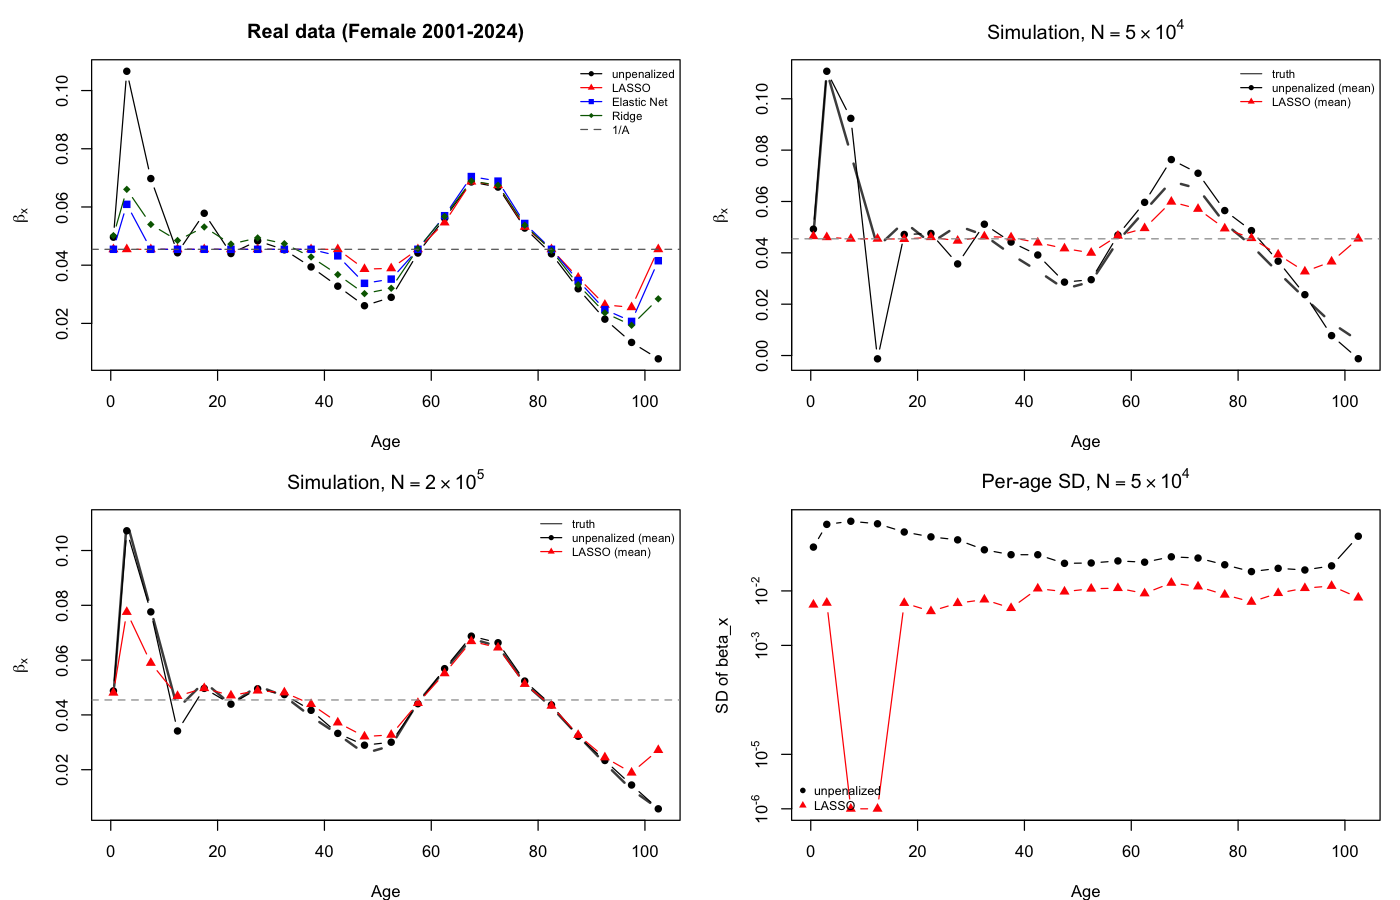
\includegraphics[width=\textwidth]{figA_beta_by_age.png}
\caption{懲罰前後 $\beta_x$ 的逐年齡比較。左上為實際資料；右上與左下為模擬的
平均估計值（含真值）；右下為逐年齡的標準差。}
\label{fig:appbeta}
\end{figure}

\subsection{模擬（已知真值）}

在模擬中可進一步把差異拆成偏誤與標準差（表~\ref{tab:appsim}）。
$N=5$ 萬、$\lambda/\lambda_{\max}=0.20$ 時，未懲罰版的平均絕對偏誤為
0.0069、平均標準差 0.0679；LASSO 則為 0.0123 與 0.0078。
亦即\textbf{標準差的中位數降幅達 75\%，與絕對偏誤增為 1.8 倍之間取得平衡}。

\begin{table}[H]
\centering
\caption{偏誤最大的五個年齡組（模擬，$N=5$ 萬，重複 100 次）}
\small
\begin{tabular}{lrrrrrr}
\toprule
年齡組 & 真值 & 未懲罰平均 & LASSO 平均 & LASSO 偏誤
& 未懲罰 SD & LASSO SD\\
\midrule
1--4   & 0.1107 & 0.1107 & 0.0461 & $-0.0646$ & 0.1666 & 0.0060\\
100+   & 0.0058 & $-0.0012$ & 0.0455 & $+0.0397$ & 0.1008 & 0.0075\\
5--9   & 0.0785 & 0.0924 & 0.0455 & $-0.0330$ & 0.1899 & 0.0000\\
95--99 & 0.0127 & 0.0078 & 0.0366 & $+0.0239$ & 0.0288 & 0.0123\\
45--49 & 0.0260 & 0.0286 & 0.0417 & $+0.0157$ & 0.0321 & 0.0097\\
\bottomrule
\end{tabular}
\label{tab:appsim}
\end{table}

\textbf{懲罰造成的偏誤集中在兩端年齡}（1--9 歲與 95 歲以上），
正是資訊量最稀薄之處；而這些年齡的未懲罰標準差高達 0.10 至 0.19，
本就不具參考價值。換言之，懲罰在這些年齡是以「明確的偏誤」取代
「無法使用的變異」，是否值得須視用途而定：
若後續要計算平均餘命（對 $\beta_x$ 的加權以死亡數為主），
兩端年齡的偏誤影響有限；若要直接解讀各年齡的改善速度，則須特別註明。

\vspace{10pt}
\section*{參考文獻}
\addcontentsline{toc}{section}{參考文獻}

\small
\noindent\textbf{一、中文部分}
\begin{itemize}[leftmargin=2em, label={}, itemsep=3pt]
  \item[] 王信忠、金碩、余清祥（2012）。小區域死亡率推估之研究。人口學刊，
        45：121-154。doi:10.6191/JPS.2012.11
  \item[] 王信忠、余清祥、王子瑜（2017）。臺灣原住民死亡率暨生命表編撰研究。
        人口學刊，55：99-131。doi:10.6191/JPS.2017.55.03
  \item[] 余清祥、王信忠、陳譽騰（2021）。年輪變動比用於小區域人口推估的探討。
        人口學刊，63：99-133。doi:10.6191/JPS.202112\_(63).0003
  \item[] 余清祥、王信忠、呂靖翎（2025）。平均餘命與標準化死亡率之相關分析。
        人口學刊，85-116。
  \item[] 陳政勳、余清祥（2010）。小區域人口推估研究：臺北市、雲嘉兩縣、
        澎湖縣的實證分析。人口學刊，41：153-183。doi:10.6191/JPS.2010.9
\end{itemize}

\vspace{4pt}
\noindent\textbf{二、英文部分}
\begin{itemize}[leftmargin=2em, label={}, itemsep=3pt]
  \item[] Alho, J. M. 1992. ``Modeling and Forecasting U.S. Mortality:
        Comment.'' \textit{Journal of the American Statistical Association}
        87(419): 673-674.
  \item[] Basellini, U., C. G. Camarda, and H. Booth. 2023. ``Thirty Years On:
        A Review of the Lee--Carter Method for Forecasting Mortality.''
        \textit{International Journal of Forecasting} 39(3): 1033-1049.
  \item[] Booth, H., J. Maindonald, and L. Smith. 2002. ``Applying Lee--Carter
        under Conditions of Variable Mortality Decline.''
        \textit{Population Studies} 56(3): 325-336.
  \item[] Booth, H., R. J. Hyndman, L. Tickle, and P. De Jong. 2006.
        ``Lee--Carter Mortality Forecasting: A Multi-country Comparison of
        Variants and Extensions.'' \textit{Demographic Research} 15: 289-310.
  \item[] Booth, H., L. Tickle, and L. Smith. 2005. ``Evaluation of the
        Variants of the Lee-Carter Method of Forecasting Mortality:
        A Multi-country Comparison.''
        \textit{New Zealand Population Review} 31(1): 13-34.
  \item[] Brouhns, N., M. Denuit, and J. K. Vermunt. 2002. ``A Poisson
        Log-bilinear Regression Approach to the Construction of Projected
        Lifetables.'' \textit{Insurance: Mathematics and Economics}
        31(3): 373-393.
  \item[] B\"uhlmann, P., and S. van de Geer. 2011. \textit{Statistics for
        High-Dimensional Data: Methods, Theory and Applications.} Springer.
  \item[] Cairns, A. J. G., D. Blake, K. Dowd, G. D. Coughlan, and
        M. Khalaf-Allah. 2011. ``Bayesian Stochastic Mortality Modelling for
        Two Populations.'' \textit{ASTIN Bulletin} 41(1): 29-59.
  \item[] Camarda, C. G., and U. Basellini. 2021. ``Smoothing, Decomposing and
        Forecasting Mortality Rates.'' \textit{European Journal of Population}
        37(3): 569-602.
  \item[] Chen, L., A. J. G. Cairns, and T. Kleinow. 2017. ``Small Population
        Bias and Sampling Effects in Stochastic Mortality Modelling.''
        \textit{European Actuarial Journal} 7(1): 193-230.
  \item[] Currie, I. D. 2011. ``Modelling and Forecasting the Mortality of the
        Very Old.'' \textit{ASTIN Bulletin} 41(2): 419-427.
  \item[] Currie, I. D. 2013. ``Smoothing Constrained Generalized Linear Models
        with an Application to the Lee--Carter Model.''
        \textit{Scandinavian Actuarial Journal} 2016(4): 356-383.
  \item[] Currie, I. D., M. Durban, and P. H. C. Eilers. 2004. ``Smoothing
        and Forecasting Mortality Rates.'' \textit{Statistical Modelling}
        4(4): 279-298.
  \item[] Delwarde, A., M. Denuit, and P. Eilers. 2007. ``Smoothing the
        Lee--Carter and Poisson Log-bilinear Models for Mortality Forecasting:
        A Penalized Log-likelihood Approach.''
        \textit{Statistical Modelling} 7(1): 29-48.
  \item[] Djeundje, V. A. B., and I. D. Currie. 2010. ``Smoothing Dispersed
        Counts with Applications to Mortality Data.''
        \textit{Annals of Actuarial Science} 5(1): 33-52.
  \item[] Dokumentov, A., R. J. Hyndman, and L. Tickle. 2018. ``Bivariate
        Smoothing of Mortality Surfaces with Zero Counts: The Lasso2d Method.''
        \textit{Stat} 7(1): e199.
  \item[] Eilers, P. H. C., and B. D. Marx. 1996. ``Flexible Smoothing with
        B-splines and Penalties.'' \textit{Statistical Science} 11(2): 89-102.
  \item[] Friedman, J., T. Hastie, and R. Tibshirani. 2010. ``Regularization
        Paths for Generalized Linear Models via Coordinate Descent.''
        \textit{Journal of Statistical Software} 33(1): 1-22.
  \item[] Hoerl, A. E., and R. W. Kennard. 1970. ``Ridge Regression: Biased
        Estimation for Nonorthogonal Problems.''
        \textit{Technometrics} 12(1): 55-67.
  \item[] Hunt, A., and D. Blake. 2020. ``Identifiability in Age/Period
        Mortality Models.'' \textit{Annals of Actuarial Science} 14(2): 461-499.
  \item[] Hunt, A., and D. Blake. 2021. ``On the Structure and Classification of
        Mortality Models.'' \textit{North American Actuarial Journal}
        25(sup1): S215-S234.
  \item[] Hyndman, R. J., and M. S. Ullah. 2007. ``Robust Forecasting of
        Mortality and Fertility Rates: A Functional Data Approach.''
        \textit{Computational Statistics \& Data Analysis} 51(10): 4942-4956.
  \item[] James, W., and C. Stein. 1961. ``Estimation with Quadratic Loss.''
        \textit{Proceedings of the Fourth Berkeley Symposium on Mathematical
        Statistics and Probability} 1: 361-379.
  \item[] Lee, R. D., and L. R. Carter. 1992. ``Modeling and Forecasting U.S.
        Mortality.'' \textit{Journal of the American Statistical Association}
        87(419): 659-671.
  \item[] Lee, R., and T. Miller. 2001. ``Evaluating the Performance of the
        Lee--Carter Method for Forecasting Mortality.''
        \textit{Demography} 38(4): 537-549.
  \item[] Jarner, S. F., and E. M. Kryger. 2011. ``Modelling Adult Mortality in
        Small Populations: The SAINT Model.''
        \textit{ASTIN Bulletin} 41(2): 377-418.
  \item[] Lee, J. D., Y. Sun, and M. A. Saunders. 2014. ``Proximal Newton-type
        Methods for Minimizing Composite Functions.''
        \textit{SIAM Journal on Optimization} 24(3): 1420-1443.
  \item[] Li, J. S.-H., M. R. Hardy, and K. S. Tan. 2009. ``Uncertainty in
        Mortality Forecasting: An Extension to the Classical Lee-Carter
        Approach.'' \textit{ASTIN Bulletin} 39(1): 137-164.
  \item[] Li, N., R. D. Lee, and S. Tuljapurkar. 2004. ``Using the Lee--Carter
        Method to Forecast Mortality for Populations with Limited Data.''
        \textit{International Statistical Review} 72(1): 19-36.
  \item[] Li, N., and R. Lee. 2005. ``Coherent Mortality Forecasts for a Group
        of Populations: An Extension of the Lee--Carter Method.''
        \textit{Demography} 42(3): 575-594.
  \item[] Lu, Y., and D. Zhu. 2023. ``Modelling Mortality: A Bayesian
        Factor-augmented VAR (FAVAR) Approach.''
        \textit{ASTIN Bulletin} 53(1): 29-61.
  \item[] Meinshausen, N. 2007. ``Relaxed Lasso.''
        \textit{Computational Statistics \& Data Analysis} 52(1): 374-393.
  \item[] Pitt, D., J. Li, and T. K. Lim. 2018. ``Smoothing Poisson Common
        Factor Model for Projecting Mortality Jointly for Both Sexes.''
        \textit{ASTIN Bulletin: The Journal of the IAA} 48(2): 509-541.
  \item[] Rabbi, A. M. F., and S. Mazzuco. 2021. ``Mortality Forecasting with
        the Lee--Carter Method: Adjusting for Smoothing and Lifespan
        Disparity.'' \textit{European Journal of Population} 37(1): 97-120.
  \item[] Renshaw, A. E., and S. Haberman. 2003. ``Lee--Carter Mortality
        Forecasting with Age-specific Enhancement.''
        \textit{Insurance: Mathematics and Economics} 33(2): 255-272.
  \item[] Santolino, M. 2020. ``The Lee-Carter Quantile Mortality Model.''
        \textit{Scandinavian Actuarial Journal} 2020(7): 614-633.
  \item[] Schuette, D. R. 1978. ``A Linear Programming Approach to
        Graduation.'' \textit{Transactions of Society of Actuaries}
        30: 407-431.
  \item[] Shang, H. L., H. Booth, and R. J. Hyndman. 2011. ``Point and Interval
        Forecasts of Mortality Rates and Life Expectancy: A Comparison of Ten
        Principal Component Methods.''
        \textit{Demographic Research} 25: 173-214.
  \item[] Stoeldraijer, L., C. van Duin, L. van Wissen, and F. Janssen. 2018.
        ``Comparing Strategies for Matching Mortality Forecasts to the Most
        Recently Observed Data.'' \textit{Genus} 74(1): 16.
  \item[] Tibshirani, R. 1996. ``Regression Shrinkage and Selection via the
        Lasso.'' \textit{Journal of the Royal Statistical Society, Series B}
        58(1): 267-288.
  \item[] Tseng, P. 2001. ``Convergence of a Block Coordinate Descent Method
        for Nondifferentiable Minimization.'' \textit{Journal of Optimization
        Theory and Applications} 109(3): 475-494.
  \item[] Wang, H. C., C. J. Yue, and C. T. Chong. 2018. ``Mortality Models and
        Longevity Risk for Small Populations.''
        \textit{Insurance: Mathematics and Economics} 78: 351-359.
  \item[] Wilmoth, J. R. 1993. \textit{Computational Methods for Fitting and
        Extrapolating the Lee--Carter Model of Mortality Change.} Technical
        Report, Department of Demography, University of California, Berkeley.
  \item[] Wi\'sniowski, A., P. W. F. Smith, J. Bijak, J. Raymer, and
        J. J. Forster. 2015. ``Bayesian Population Forecasting: Extending the
        Lee--Carter Method.'' \textit{Demography} 52(3): 1035-1059.
  \item[] Yang, S. S., J. C. Yue, and H. C. Huang. 2010. ``Modeling Longevity
        Risks Using a Principal Component Approach: A Comparison with Existing
        Stochastic Mortality Models.''
        \textit{Insurance: Mathematics and Economics} 46(1): 254-270.
  \item[] Yue, J. C., H. C. Wang, and T. Y. Wang. 2019. ``Using Graduation to
        Modify the Estimation of Lee--Carter Model for Small Populations.''
        \textit{North American Actuarial Journal}.
        doi:10.1080/10920277.2019.1650288
  \item[] Zhang, L., and Y. Zhuang. 2026. ``What KAN Mortality Say: Smooth and
        Interpretable Mortality Modeling Using Kolmogorov--Arnold Networks.''
        \textit{ASTIN Bulletin} 56(1): 32-59.
  \item[] Zhang, C.-H. 2010. ``Nearly Unbiased Variable Selection under
        Minimax Concave Penalty.'' \textit{The Annals of Statistics}
        38(2): 894-942.
  \item[] Zou, H. 2006. ``The Adaptive Lasso and Its Oracle Properties.''
        \textit{Journal of the American Statistical Association}
        101(476): 1418-1429.
  \item[] Zou, H., and T. Hastie. 2005. ``Regularization and Variable Selection
        via the Elastic Net.'' \textit{Journal of the Royal Statistical
        Society, Series B} 67(2): 301-320.
\end{itemize}

\end{document}
